\documentclass[12pt,a4paper]{book}
\usepackage[utf8]{inputenc}
\usepackage[T1]{fontenc}
\usepackage[a4paper, left=3cm, right=2.5cm, top=2.5cm, bottom=3cm]{geometry}

\usepackage{graphicx}
\usepackage{fancyhdr}
\usepackage{setspace}
\usepackage{amsmath}
\usepackage{mathtools}
\usepackage{amssymb}
\usepackage{amsthm}
\usepackage{pdfpages}
\usepackage{enumitem}
\usepackage{emptypage}
\usepackage[most]{tcolorbox}
\usepackage{url}
\overfullrule=2pt

\usepackage[spanish]{babel}

\renewcommand{\sin}{\operatorname{sen}}
\renewcommand{\arcsin}{\operatorname{arcsen}}
\renewcommand{\Re}{\operatorname{Re}}

\pagestyle{fancy}

\newtheorem{theorem}{Teorema}
\newtheorem{definition}[theorem]{Definición}
\newtheorem{lemma}[theorem]{Lema}
\newtheorem{corollary}[theorem]{Corolario}
\newtheorem{prop}[theorem]{Proposición}

\title{TFG - La función hipergeométrica de Gauss}
\author{Daniel González}
\date{2025--2026}

\setlength{\headheight}{28pt}

\usepackage{hyperref}

\begin{document}


\includepdf[pages=-, fitpaper]{portada.pdf}

\newpage
\thispagestyle{empty}
\null
\newpage

\begin{titlepage}
    \centering
    \vspace*{1cm}
    
    % Título del trabajo
    {\Huge \setstretch{1.2} \textbf{La función hipergeométrica de Gauss}\par}
    
    \vspace{1.5cm}
    {\Large Trabajo de Fin de Grado\par}
    \vfill
    
    % Ilustración/Imagen (puedes cambiar a gauss.jpg si lo prefieres)
    % El paquete graphicx debe estar cargado en tu preámbulo
    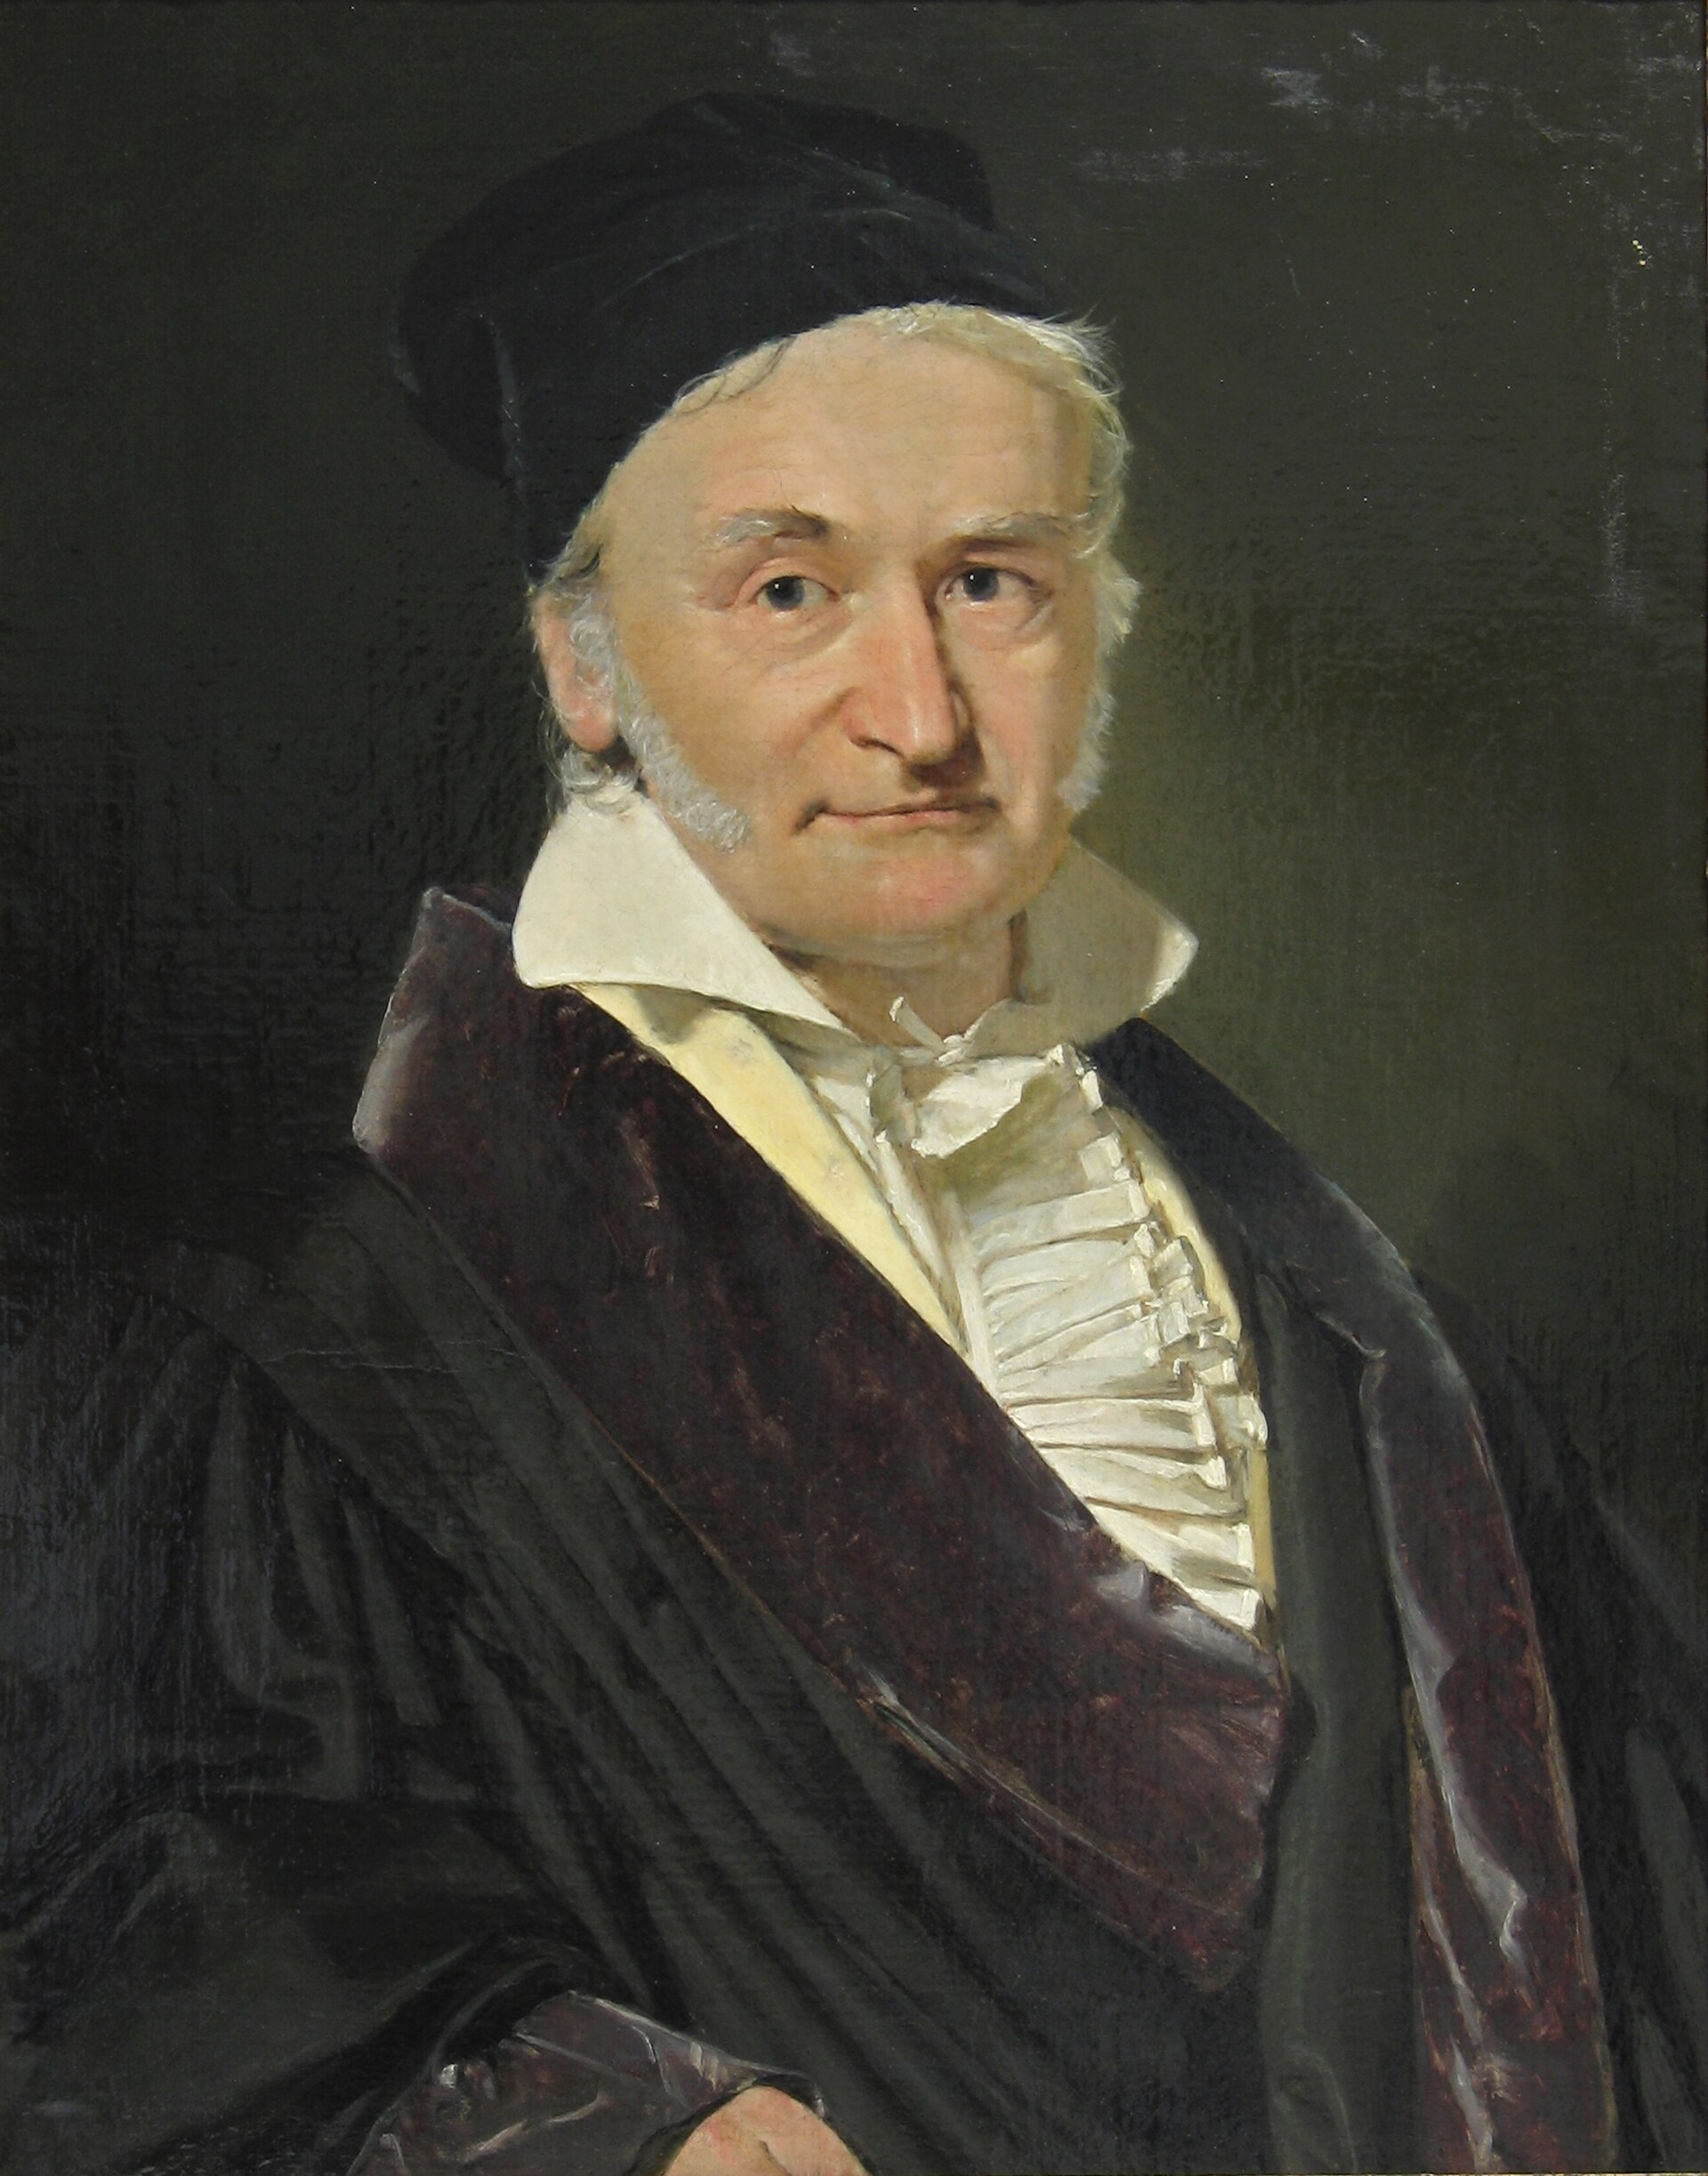
\includegraphics[width=0.5\textwidth]{gauss.jpg}
    
    \vfill
    \vspace{2cm}
    
    % Bloque de Autor y Tutor alineados en paralelo
    \noindent
    \begin{minipage}[t]{0.45\textwidth}
        \begin{flushleft} \large
            \textbf{Autor} \\
            Daniel González Espinosa
        \end{flushleft}
    \end{minipage}
    \hfill
    \begin{minipage}[t]{0.45\textwidth}
        \begin{flushright} \large
            \textbf{Tutor} \\
            Óscar Ciaurri Ramírez
        \end{flushright}
    \end{minipage}
    
    \vfill
    \vspace{1cm}
    
    % Ubicación y Fecha
    {\large Logroño, junio de 2026\par}
\end{titlepage}

\newpage
\thispagestyle{empty}
\null
\newpage

\newpage
\thispagestyle{empty}
\begin{flushleft}
    {\Large \textbf{Resumen}}
\end{flushleft}
Este trabajo de fin de grado presenta un estudio analítico y global de la función hipergeométrica de Gauss, destacando su relevancia como marco unificador dentro de la teoría de las funciones especiales. De manera general, se aborda la construcción teórica de esta función, explorando desde su convergencia y su extensión analítica al plano complejo, hasta su profunda relación estructural con las familias de polinomios ortogonales clásicos, tales como los de Jacobi. Además de recopilar y probar sus propiedades, representaciones integrales y transformaciones algebraicas, el trabajo culmina con una aportación matemática propia, el desarrollo de identidades hipergeométricas originales. En conjunto, el documento ilustra el enorme potencial analítico de la función hipergeométrica, tanto para generalizar resultados como para descubrir nuevas relaciones matemáticas.

\vspace{1.5cm} 

\selectlanguage{english}

\begin{flushleft}
    {\Large \textbf{Abstract}}
\end{flushleft}
This project presents a comprehensive analytical study of the Gauss hypergeometric function, highlighting its significance as a unifying framework within the theory of special functions. In general terms, it addresses the theoretical construction of this function, exploring everything from its convergence and its analytic extension in the complex plane to its deep structural relationship with families of classical orthogonal polynomials, such as those of Jacobi. In addition to compiling and proving its properties, integral representations and algebraic transformations, the project culminates in a personal mathematical contribution, the development of original hypergeometric identities. Taken as a whole, the project illustrates the immense analytical potential of the hypergeometric function, both for generalising results and for discovering new mathematical relationships.

\selectlanguage{spanish}

\newpage
\thispagestyle{empty}
\null
\newpage

\renewcommand{\contentsname}{Índice general}
\renewcommand{\chaptername}{Capítulo}
\renewcommand{\proofname}{Demostración}



\tableofcontents 
\newpage
\thispagestyle{empty} 

\cleardoublepage
\markboth{}{} 
\chapter*{Introducción}
\addcontentsline{toc}{chapter}{Introducción}
\thispagestyle{plain} 
La función hipergeométrica de Gauss representa uno de los objetos analíticos más robustos y versátiles dentro de la teoría de las funciones especiales y el análisis complejo. Su enorme valor matemático radica en su capacidad para unificar una vasta gama de funciones elementales y trascendentes (como la función logaritmo, el arcoseno, la serie binomial o las integrales elípticas) mediante una elección adecuada de sus parámetros.

El estudio de esta función hunde sus raíces en los albores del cálculo. El término «serie hipergeométrica» fue introducido por primera vez en 1655 por el matemático inglés John Wallis en su obra \textit{Arithmetica Infinitorum}. A mediados del siglo XVIII, Leonhard Euler (1748) realizó un escrutinio analítico de estas series y dedujo representaciones integrales fundamentales. Sin embargo, el primer tratamiento sistemático y riguroso en el dominio complejo fue proporcionado por Carl Friedrich Gauss en su célebre tratado \textit{Disquisitiones generales circa seriem infinitam} de 1812 (publicado en 1813), lo que dio nombre a la función que hoy conocemos. El desarrollo de la teoría continuó durante el siglo XIX con las aportaciones de Ernst Kummer en 1836, quien descubrió profundas fórmulas de transformación, y alcanzó su madurez geométrica con Bernhard Riemann en 1857, quien caracterizó la función hipergeométrica de manera definitiva a través de la ecuación diferencial de segundo orden que satisface y sus tres singularidades regulares.

Este trabajo de fin de grado aborda un estudio analítico y detallado de esta función y se estructura en tres capítulos fundamentales, abarcando desde sus propiedades teóricas básicas hasta el desarrollo de identidades originales.

En el Capítulo 1 se establecen los fundamentos analíticos de la función hipergeométrica. Se parte de su definición formal mediante una serie de potencias utilizando el símbolo de Pochhammer. A continuación, se realiza un estudio riguroso de la convergencia de la serie; no solo se demuestra que su radio de convergencia es el disco unidad mediante el criterio del cociente, sino que se caracteriza exhaustivamente su comportamiento en la propia frontera del disco empleando la fórmula asintótica de Stirling y el criterio de Dirichlet. Posteriormente, se introduce la representación integral de Euler, una herramienta clave que permite demostrar, mediante el principio de prolongación analítica, cómo la función puede extenderse de forma única a casi todo el plano complejo. El capítulo finaliza con el estudio de algunas transformaciones lineales y la evaluación exacta de la función en puntos especiales.

El Capítulo 2 está dedicado a explorar la profunda conexión existente entre la función hipergeométrica y la teoría de los polinomios ortogonales clásicos. El capítulo se centra en los polinomios de Jacobi, que se introducen a través de la fórmula de Rodrigues. Se deduce la ecuación diferencial lineal de segundo orden que estos satisfacen y se demuestra un resultado clave: mediante un adecuado cambio de variable lineal, dicha ecuación se transforma en la ecuación hipergeométrica, lo que permite representar los polinomios de Jacobi como una serie hipergeométrica truncada. A partir de este marco general, se analizan como casos particulares importantes los polinomios de Gegenbauer (o ultraesféricos) y los polinomios de Legendre. Finalmente, se demuestra formalmente la ortogonalidad de la familia de Jacobi con respecto a su función peso, calculando su norma, y se deriva la eficiente relación de recurrencia a tres términos para su evaluación.

El Capítulo 3 culmina el trabajo con el estudio y desarrollo de identidades hipergeométricas. El punto de partida de este capítulo está motivado por un problema geométrico reciente que vincula el área de los sectores de una curva de Lamé con la longitud de arco de una espiral sinusoidal. Esta correspondencia inspira la definición de una familia general de integrales. Tras utilizar estos resultados para demostrar identidades hipergeométricas previamente conocidas relacionadas con transformaciones cuadráticas clásicas, el capítulo presenta nuevas aportaciones originales que no se encuentran en la literatura estándar de funciones especiales. Estas nuevas identidades se obtienen aplicando el teorema del binomio de Newton generalizado sobre diversos factores del integrando. El resultado es una serie de teoremas que logran expandir integrales hipergeométricas complejas en forma de series infinitas de nuevas funciones hipergeométricas evaluadas en argumentos cuadráticos y cuárticos.

\fancypagestyle{intro}{
    \fancyhf{}
    \fancyhead[LE]{\thepage}
    \fancyhead[RE]{\textit{Introducción}}
    \fancyhead[LO]{\textit{Introducción}}
    \fancyhead[RO]{\thepage}
    \renewcommand{\headrulewidth}{0.4pt}
    \renewcommand{\footrulewidth}{0pt}
}
\pagestyle{intro}


\newpage
\thispagestyle{empty} 

\fancyhf{} 
\fancyhead[LE]{\thepage}
\fancyhead[RE]{\textit{\nouppercase{\leftmark}}}
\fancyhead[RO]{\thepage}
\fancyhead[LO]{\textit{\nouppercase{\rightmark}}}
\renewcommand{\headrulewidth}{0.4pt}
\renewcommand{\footrulewidth}{0pt}
\makeatletter
\renewcommand{\chaptermark}[1]{%
  \markboth{Capítulo \thechapter. \ #1}{}}
\renewcommand{\sectionmark}[1]{%
  \markright{\thesection. \ #1}}
\makeatother


\chapter[Definición y primeras propiedades]{La función hipergeométrica de Gauss: definición y primeras propiedades}
\label{chap:funcion_hipergeometrica}

En este capítulo sentaremos las bases para el estudio de la función que nos ocupa. Comenzamos con su definición formal a través de una serie de potencias, que es el punto de partida histórico y conceptual para entender su comportamiento. Analizaremos sus parámetros, su radio de convergencia y daremos una representación integral para la misma, la cual nos permitirá dar su extensión analítica a casi todo el plano complejo.

\section{Definición}
\label{sec:definicion_propiedades}

\begin{definition}[Función hipergeométrica de Gauss]
Dados tres parámetros complejos $a, b, c \in \mathbb{C}$ y una variable compleja $z$, la función hipergeométrica de Gauss, denotada como ${}_{2}F_{1}(a,b;c;z)$, se define mediante la serie de potencias
\[
{}_{2}F_{1}(a,b;c;z) = \sum_{n=0}^{\infty} \frac{(a)_n (b)_n}{(c)_n} \frac{z^n}{n!},
\]
donde $(x)_n$ es el símbolo de Pochhammer definido como
\[
(x)_n = 
\begin{cases}
1, & \text{si } n=0, \\
x(x+1)(x+2)\cdots(x+n-1), & \text{si } n > 0.
\end{cases}
\]
\end{definition}
El símbolo de Pochhammer también puede expresarse de forma compacta utilizando la función gamma de Euler como $(x)_n = \Gamma(x+n)/\Gamma(x)$, cuando $x \in \mathbb{C} \setminus \{0,-1,-2,\dots\} $.

La función hipergeométrica depende de una variable y tres parámetros, sujetos a las siguientes condiciones:
\begin{itemize}

    \item Los parámetros $a$ y $b$ pueden ser cualesquiera números complejos. La función es simétrica con respecto a estos dos parámetros. Esto es evidente a partir de la propia definición de la serie y se tiene
    \[
    {}_{2}F_{1}(a,b;c;z) = {}_{2}F_{1}(b,a;c;z).
    \]
    Una de las propiedades más interesantes de la función es que, bajo ciertas condiciones, la serie infinita se trunca y se convierte en un polinomio. Esto ocurre cuando el parámetro $a$ o $b$ (o ambos) es un entero no positivo.
    Por ejemplo, si $a = -m$ para algún entero $m \geq 0$, el símbolo de Pochhammer $(-m)_n$ se anula para todo $n > m$ y se verifica
    \[ (-m)_n = (-m)(-m+1)\cdots(-m+n-1) = 0, \quad  n=m+1, m+2, \dots\,.\]
    Esto provoca que todos los coeficientes de la serie a partir del término $n=m+1$ sean cero. La serie se reduce a una suma finita, dando lugar a un polinomio de grado $m$ en $z$
    \[
    {}_{2}F_{1}(-m,b;c;z) = \sum_{n=0}^{m} \frac{(-m)_n (b)_n}{(c)_n} \frac{z^n}{n!}.
    \]
    Este hecho es fundamental, ya que conecta la función hipergeométrica con familias de polinomios ortogonales, como los de Jacobi, Gegenbauer y Legendre, que serán objeto de estudio en el Capítulo 2.
    \item El parámetro $c$ puede ser cualquier número complejo, con la crucial excepción de los enteros no positivos ($c \neq 0, -1, -2, \dots$). Esta restricción es necesaria porque si $c$ tomara uno de estos valores, el símbolo de Pochhammer $(c)_n$ se anularía para algún $n$, provocando una división por cero en los coeficientes de la serie. Esto se puede solucionar tomando una versión regularizada de la función
    \[
    {}_{2}\tilde{F}_{1}(a,b;c;z) =
    \frac{{}_{2}F_{1}(a,b;c;z)}{\Gamma(c)}, 
    \]
    cuyos valores cuando \(c = 0,-1,-2,\dots\) se definen mediante el límite
    \[
    {}_{2}\tilde{F}_{1}(a,b;c;z) =
    \lim_{c' \to c} \frac{{}_{2}F_{1}(a,b;c';z)}{\Gamma(c')} = \lim_{c' \to c} \sum_{n=0}^{\infty} \frac{(a)_n (b)_n}{\Gamma(c'+n)} \frac{z^n}{n!}.
    \]
\end{itemize}

\subsubsection*{Ejemplos: Funciones elementales como casos particulares de la función hipergeométrica de Gauss}

La gran generalidad de la función ${}_{2}F_{1}$ permite expresar un número sorprendente de funciones matemáticas conocidas simplemente eligiendo los parámetros $a, b$ y $c$ de forma adecuada. A continuación se muestran algunos ejemplos notables.

\begin{itemize}
    \item La serie geométrica. Puesto que $(1)_n = n!$, es claro que
    \[ {}_{2}F_{1}(1,b;b;z) = \sum_{n=0}^{\infty} \frac{(1)_n (b)_n}{(b)_n} \frac{z^n}{n!} = \sum_{n=0}^{\infty} z^n = \frac{1}{1-z}, \quad |z|<1. \]
    En efecto, esta conexión es el origen del nombre hipergeométrica.  


    \item La serie binomial. Como $(-a)_n = (-a)(-a+1)\cdots(-a+n-1) = (-1)^n a(a-1)\cdots(a-n+1)$ se tiene que
    \[
    \frac{(-a)_n}{n!}= (-1)^n \binom{a}{n},
    \]
    y aplicando el binomio de Newton
    \[ {}_{2}F_{1}(-a,b;b;-z) = \sum_{n=0}^{\infty} \frac{(-a)_n (b)_n}{(b)_n}\frac{(-z)^n}{n!} = \sum_{n=0}^{\infty}\binom{a}{n} z^n = (1+z)^a,\]
    si $|z|<1$.

    \item La función logaritmo. Usando la identidad $(2)_n = (n+1)!$,\footnote{En general, si $m \in \mathbb{N}$ se verifica que $(m)_n = (m+n-1)!/(m-1)!$.} deducimos que 
    \[ z \cdot {}_{2}F_{1}(1,1;2;-z) = z \sum_{n=0}^{\infty} \frac{((1)_n)^2}{(2)_n}\frac{(-z)^n}{n!} = \sum_{n=0}^{\infty} \frac{(-1)^n z^{n+1}}{n+1} = \log(1+z), \]
    cuando $|z|<1$.

    \item La función arcoseno. De las relaciones 
    \begin{equation}
    \label{eq1}
        \left(\frac{1}{2}\right)_n = \frac{1}{2n+1} \left(\frac{3}{2}\right)_n
    \end{equation}
    y
    \begin{equation}
    \label{eq2}
    \begin{aligned}
        \frac{(1/2)_n}{n!} &= \frac{\Gamma(n+1/2)}{n! \, \Gamma(1/2)} =  \frac{(n-1/2)(n-3/2) \cdots (1/2)\Gamma(1/2)}{n! \, \Gamma(1/2)} \\
        &= \frac{(-1)^n(-1/2)(-3/2) \cdots (-1/2 -n +1)}{n!} \\&= (-1)^n \binom{-1/2}{n},
    \end{aligned}
\end{equation}
    concluimos que 
    \begin{align*}
      z \cdot {}_{2}F_{1}\left(\frac{1}{2}, \frac{1}{2}; \frac{3}{2}; z^2\right) &= z \sum_{n=0}^{\infty} \frac{((1/2)_n)^2}{(3/2)_n}\frac{z^{2n}}{n!} = \sum_{n=0}^{\infty}\binom{-1/2}{n} \frac{(-1)^n z^{2n+1}}{2n+1} \\ &= \int_0^z \sum_{n=0}^\infty \binom{-1/2}{n} (-1)^nt^{2n} \, dt= \int_0^z\frac{dt}{\sqrt{1-t^2}} \\ &=  \arcsin z,  
    \end{align*}
    donde suponemos $|z|<1$. El intercambio de la suma y la integral en la prueba anterior puede justificarse por el teorema de la convergencia uniforme.

    \item La integral elíptica completa de primera especie. Dado $0 \leq k <1$, definimos la integral elíptica de primera especie como
    \[K(k)= \int_{0}^{\pi/2} \frac{d\theta}{\sqrt{1-k^2 \sin^{2}{\theta}}}.\]
    Así, aplicando \eqref{eq2} y la relación
    \[\int_{0}^{\pi/2} \sin^{2n}\theta \, d\theta = \frac{1}{2} B(n+1/2, 1/2) = \frac{1}{2}\frac{\Gamma(n+ 1/2)\Gamma(1/2)}{\Gamma(n+1)} = \frac{\pi}{2}\frac{(1/2)_n}{n!},\]
    obtenemos que
    \begin{align*}
    \frac{\pi}{2} \cdot {}_{2}F_{1}\left(\frac{1}{2}, \frac{1}{2}; 1; k^2\right) &= \frac{\pi}{2} \sum_{n=0}^{\infty} \frac{{(1/2)_n}^2}{(n!)^2}k^{2n} \\ &=  \sum_{n=0}^{\infty} (-1)^n \binom{-1/2}{n}\int_{0}^{\pi/2} (k^2 \sin^2\theta)^n \,d\theta \\ &= \int_{0}^{\pi/2}\sum_{n=0}^{\infty} (-1)^n \binom{-1/2}{n}(k^2 \sin^2\theta)^n \, d\theta \\ &= \int_{0}^{\pi/2} \frac{d\theta}{\sqrt{1-k^2 \sin^{2}{\theta}}} = K(k),
    \end{align*}
    donde en esta ocasión el intercambio de la suma y la integral puede justificarse por el teorema de la convergencia monótona ya que $(-1)^n \binom{-1/2}{n} > 0$. Para un análisis más exhaustivo de las integrales elípticas se pueden consultar \cite{ortega} y \cite{puron}.
    
\end{itemize}
Estos ejemplos ilustran que la función hipergeométrica de Gauss no es una mera curiosidad matemática, sino un marco unificador para muchas funciones previamente conocidas.

\section{Convergencia de la serie hipergeométrica}
\label{sec:convergencia}

Una vez definida la función hipergeométrica a través de su serie de potencias, el primer paso fundamental en su análisis es determinar su dominio de validez. En esta sección estudiaremos en detalle su radio de convergencia y, de forma más sutil, su comportamiento en la frontera de dicho dominio.

\subsection{Convergencia en el disco unidad}

El radio de convergencia de la serie se establece de manera directa mediante el criterio del cociente, que nos proporciona un resultado claro sobre el dominio donde la función está bien definida.

\begin{theorem}[Radio de convergencia]
La serie hipergeométrica ${}_{2}F_{1}(a,b;c;z)$ converge absolutamente para $|z|<1$ y diverge para $|z|>1$. Es decir, su radio de convergencia es $R=1$.
\end{theorem}

\begin{proof}
Denominamos $T_n$ al término $n$-ésimo de la serie que define la función ${}_{2}F_{1}(a,b;c;z)$. Para aplicar el criterio del cociente, calculamos el límite del valor absoluto del cociente de dos términos consecutivos
\[
L = \lim_{n \to \infty} \left| \frac{T_{n+1}}{T_n} \right| = \lim_{n \to \infty} \left| \frac{(a)_{n+1} (b)_{n+1} z^{n+1}}{(c)_{n+1} (n+1)!} \cdot \frac{(c)_n n!}{(a)_n (b)_n z^n} \right|.
\]
Utilizando la propiedad $(x)_{n+1} = (x)_n (x+n)$, podemos simplificar la expresión para obtener
\[
L = \lim_{n \to \infty} \left| \frac{(a+n)(b+n)}{(c+n)(n+1)} z \right| = |z|.
\]
Según el criterio del cociente, la serie converge absolutamente si este límite $L$ es menor que uno, es decir, si $|z|<1$, y diverge si es mayor que uno, es decir, si $|z|>1$. Esto demuestra que el radio de convergencia es $R=1$.
\end{proof}

El análisis para el caso $|z|=1$, la frontera del disco de convergencia, es más delicado y requiere herramientas más avanzadas.

\subsection{Convergencia en la frontera}

Para estudiar el comportamiento de la serie en el círculo unidad, necesitamos conocer el comportamiento asintótico de los coeficientes para $n$ grande. La herramienta clave para ello es la fórmula de Stirling para la función Gamma.

Para valores grandes de $z$, la función Gamma puede ser aproximada asintóticamente por la fórmula de Stirling
\[ \Gamma(z) \sim \sqrt{2\pi} \, z^{z - 1/2} e^{-z},\]
donde el símbolo $\sim$ indica que el cociente de ambas expresiones tiende a uno cuando $z$ tiende a infinito en el sector $|\arg z| < \pi$.
De esta fórmula deriva la conocida equivalencia de Stirling $ n!\sim \sqrt {2\pi n}(n/e)^{n} $ y usándola, podemos deducir un lema fundamental sobre el comportamiento asintótico del cociente de dos funciones Gamma.

\begin{lemma}
\label{lema:gamma_asintotico}
Sean $p, q$ números complejos fijos. Entonces
\[
\frac{\Gamma(n+q)}{\Gamma(n+p)} \sim n^{q-p} \left(1 + \frac{(q-p)(q+p-1)}{2n} \right).
\]
\end{lemma}
\begin{proof}
Aplicando la fórmula de Stirling
\[
\frac{\Gamma(n+q)}{\Gamma(n+p)} \sim \frac{\sqrt{2\pi} \, e^{-(n+q)} (n+q)^{n+q-1/2}}{\sqrt{2\pi} \, e^{-(n+p)} (n+p)^{n+p-1/2}} = e^{p-q} \cdot \frac{(n+q)^{n+q-1/2}}{(n+p)^{n+p-1/2}}.
\]
Separamos el término de las potencias en dos partes para un análisis más sencillo
\[
\frac{(n+q)^{n+q-1/2}}{(n+p)^{n+p-1/2}} = \frac{(n+q)^{n+q}}{(n+p)^{n+p}} \cdot \frac{(n+q)^{-1/2}}{(n+p)^{-1/2}}.
\]
Es fácil comprobar que
\[
\frac{(n+q)^{n+q}}{(n+p)^{n+p}} = n^{q-p} \frac{(1+q/n)^{n+q}}{(1+p/n)^{n+p}} = n^{q-p} \frac{\exp((n+q)\log(1+q/n))}{\exp((n+p)\log(1+p/n))}.
\]
Ahora, usando el desarrollo $\log(1+x) = x - x^2/2 + O(x^3)$, se llega a
\[
(n+q)\log\left(1+\frac{q}{n}\right) =
(n+q)\left(\frac{q}{n} - \frac{q^2}{2n^2} + O\left(\frac{1}{n^3}\right)\right) = q + \frac{q^2}{2n} + O\left(\frac{1}{n^2}\right),
\]
y lo análogo para $(n+p)\log(1+p/n)$.
De este modo, aplicando que $ \exp(x) = 1 + x + O(x^2)$, 
\begin{align*}
    n^{q-p} \frac{\exp(q + q^2/(2n) + O\left(\frac{1}{n^2}\right))}{\exp(p + p^2/(2n) + O\left(\frac{1}{n^2}\right))} &= n^{q-p} e^{q-p} \exp\left(\left(\frac{q^2 -p^2}{2n}\right) + O\left(\frac{1}{n^2}\right)\right) \\
    &= n^{q-p} e^{q-p} \left(\left(1 + \frac{q^2-p^2}{2n}\right) + O\left(\frac{1}{n^2}\right)\right).
\end{align*}
Para el segundo cociente, usando que 
\[
\frac{n+q}{n+p} = 1+ \frac{q-p}{n} + O\left(\frac{1}{n^2}\right)
\]
y $(1+x)^\alpha = 1+\alpha x +O(x^2)$ obtenemos que
\[
\left(\frac{n+q}{n+p}\right)^{-1/2} = 1+\frac{p-q}{2n} + O\left(\frac{1}{n^2}\right).
\]
Por tanto,
\begin{align*}
   \frac{\Gamma(n+q)}{\Gamma(n+p)} &\sim 
    e^{p-q} \cdot n^{q-p} e^{q-p} \left( 1 + \frac{q^2-p^2}{2n} \right) \cdot \left(1 + \frac{p-q}{2n}\right) \\ &=
    n^{q-p}\left(1 + \frac{q^2-q-p^2+p}{2n}\right) = n^{q-p}\left(1 + \frac{(q-p)(q+p-1)}{2n}\right). 
    \qedhere
\end{align*}
\end{proof}

Este lema nos proporciona no solo el término dominante del cociente, que es $n^{q-p}$, sino también el primer término de corrección, permitiendo un análisis de mayor precisión.

Con este resultado, podemos encontrar el comportamiento detallado del coeficiente $u_n$ de la serie hipergeométrica
\[
u_n = \frac{(a)_n (b)_n}{(c)_n n!} = \frac{\Gamma(c)}{\Gamma(a)\Gamma(b)} \cdot \frac{\Gamma(n+a)\Gamma(n+b)}{\Gamma(n+1)\Gamma(n+c)}.
\]
Aplicando el Lema \ref{lema:gamma_asintotico} a los cocientes $\Gamma(n+a)/\Gamma(n+1)$ y $\Gamma(n+b)/\Gamma(n+c)$, y multiplicando sus expresiones, obtenemos
\[
u_n \sim \frac{\Gamma(c)}{\Gamma(a)\Gamma(b)} \cdot n^{a+b-c-1} \left(1 + \frac{K}{n} \right),
\]
donde $K$ es una constante que depende de $a, b$ y $c$. Lo crucial es que el término general $T_n = u_n z^n$ se puede descomponer asintóticamente como suma de dos términos
\begin{equation}
\label{eq3}
   T_n \sim C_1 n^{a+b-c-1} z^n + C_2 n^{a+b-c-2} z^n, 
\end{equation}
donde $C_1$ y $C_2$ son ciertas constantes que dependen de $a, b$ y $c$. La convergencia en $|z|=1$ de la función hipergeométrica la obtendremos como consecuencia del siguiente resultado extraído de  \cite[pág.~243]{bromwich}.

\begin{lemma}[Criterio de Dirichlet para series complejas]
\label{lema:dirichlet_complejo}
Sean $\{a_n\}_{n \geq 0}$ y $\{b_n\}_{n \geq 0}$ dos sucesiones de números complejos tales que
\begin{enumerate} [label=\alph*)]
    \item las sumas parciales $\sum_{n=0}^N a_n$ están acotadas para todo $N \ge 0$,
    \item la serie $\sum_{n=0}^\infty (b_n - b_{n+1})$ es absolutamente convergente, y
    \item $\lim_{n \to \infty} b_n = 0$,
\end{enumerate}
entonces la serie $\sum_{n=0}^\infty a_n b_n$ converge.
\end{lemma}

Este criterio es fundamental porque nos permite garantizar la convergencia de series cuyos términos no convergen absolutamente, basándose en las cancelaciones producidas por una parte oscilatoria acotada. Generalmente, esta herramienta es la llave maestra para demostrar la convergencia condicional\footnote{Recordemos que una serie converge condicionalmente si $\sum_{n=0}^\infty c_n$ converge, pero $\sum_{n=0}^\infty |c_n|$ diverge. El ejemplo clásico son las series  de término general $c_n = (-1)^n/n^p$ con $0 < p \le 1$.} de una serie. Con este resultado, ya estamos en disposición de caracterizar por completo la convergencia en la frontera.

\begin{theorem}[Convergencia en la frontera]
\label{teo:convergencia_frontera}
Sea $\delta = \Re(c-a-b)$. Entonces en el círculo unidad, $|z|=1$, la serie hipergeométrica ${}_{2}F_{1}(a,b;c;z)$
\begin{enumerate}[label=\alph*)]
    \item converge absolutamente si $\delta > 0$,
    \item converge condicionalmente si $z \neq 1$ y $-1 < \delta \leq 0$, y
    \item diverge si $\delta \leq -1$. 
\end{enumerate}
La serie también diverge en $z=1$ si $\delta \leq 0$.
\end{theorem}

\begin{proof}
La convergencia de la serie hipergeométrica en $|z|=1$ se determina analizando la convergencia de las series obtenidas a partir de la asintótica \eqref{eq3}.

\begin{enumerate}[label=\alph*)]
    \item Caso $\delta > 0$. Por \eqref{eq3} se tiene que
    \[
    \sum_{n=1}^\infty |T_n| \leq C_1 \sum_{n=1}^\infty n^{-\delta-1} +C_2\sum_{n=1}^\infty n^{-\delta-2} \le C\sum_{n=1}^\infty n^{-\delta -1},
    \]
    y esta serie es convergente por ser $\delta >0$.
    \item Caso $-1 < \delta \leq 0$ y $z \neq 1$. Tomando $z = e^{i\theta}$, con $\theta \neq 0$, se verifica que 
    \[
    \sum_{n=1}^\infty T_n \sim C_1 \sum_{n=1}^\infty n^{-(c-a-b)-1} e^{in\theta} + C_2 \sum_{n=1}^\infty n^{-(c-a-b)-2} e^{in\theta}.
    \]
    La segunda de estas series es absolutamente convergente ya que $-1 < \delta \leq 0$. Para analizar la primera de ellas usaremos el criterio de Dirichlet (Lema \ref{lema:dirichlet_complejo}). Tomamos $a_n = e^{in\theta}$ y $b_n = n^{-(c-a-b)-1}$ y así
    \[
    \sum_{n=1}^\infty n^{-(c-a-b)-1} e^{in\theta} = \sum_{n=1}^\infty a_n b_n.
    \]
    Como 
    \[
    \left|\sum_{n=1}^N a_n \right|=\left|\sum_{n=1}^N e^{in\theta}\right|= \left|e^{i\theta}\frac{1-e^{iN\theta}}{1-e^{i\theta}}\right| \le \frac{2}{|1-e^{i\theta}|},
    \]
    la condición a) del criterio de Dirichlet se verifica. La condición c) es clara ya que $-1 < \delta \le 0$ y, como
    \begin{align*}
      b_n - b_{n+1} &= n^{-(c-a-b)-1}\left(1 - \left( 1 + \frac{1}{n}\right)^{-(c-a-b)-1}\right) \\ &\sim n^{-(c-a-b)-2}(c-a-b+1),  
    \end{align*}
    deducimos que
    \[
    \sum_{n=1}^\infty |b_n - b_{n+1}| \sim C \sum_{n=1}^\infty n^{-\delta-2} < \infty,
    \]
    por lo que también se cumple la condición b) y la serie es condicionalmente convergente.
    \item Caso $\delta \leq -1$. En esta situación, de \eqref{eq3} podemos deducir que
    \[
    \lim_{n \to \infty} |T_n| \neq 0,
    \]
    y, por tanto, la serie diverge.
\end{enumerate}
Finalmente, si $z=1$ y $-1 < \delta \le 0$ tenemos que 
\[
\sum_{n=1}^\infty T_n \sim C_1 \sum_{n=1}^\infty n^{-(c-a-b)-1} + C_2 \sum_{n=1}^\infty n^{-(c-a-b)-2}.
\]
La segunda de estas series es convergente pero la primera es divergente por ser $-1 < \delta \le 0$.
\end{proof}

Con este análisis, el dominio de convergencia de la serie que define la función hipergeométrica queda completamente caracterizado. Hemos demostrado que la definición de la función no se limita al disco abierto $|z|<1$, sino que se extiende de forma muy precisa a la frontera. El valor de $\Re(c-a-b)$ actúa como un árbitro que decide el comportamiento de la serie en el círculo unidad, determinando si converge absoluta o condicionalmente, o si diverge.


\section{La representación integral y la extensión analítica}
\label{sec:representacion_integral}

La definición de la función hipergeométrica de Gauss como serie de potencias es el punto de partida natural para su estudio. Sin embargo, como hemos demostrado, esta definición está limitada a un dominio $D_S = \{z \in \mathbb{C} : |z| < 1\}$. Fuera de este disco, la serie diverge.

El objetivo de esta sección es introducir una función integral, $I(z)$, y demostrar formalmente que es la prolongación analítica única de la serie de potencias a casi todo el plano complejo. 
Introducimos, por tanto, un candidato para esta prolongación analítica, la función $I(z)$ definida por la integral
\[
I(z)= \frac{\Gamma(c)}{\Gamma(b)\Gamma(c-b)} \int_0^1 t^{b-1} (1-t)^{c-b-1} (1-zt)^{-a} \,dt.
\]

Ahora debemos probar que esta función $I(z)$ es idéntica a nuestra función serie original dentro del disco unidad. Esto establecerá $I(z)$ como la prolongación analítica de ${}_{2}F_{1}(a,b;c;z)$.

\begin{theorem}[Representación integral de Euler]
\label{teo:representacion_integral_euler}
Para $\Re(c) > \Re(b) > 0$ y en el dominio $D_S = \{z \in \mathbb{C} : |z| < 1\}$, la función hipergeométrica de Gauss y la función integral $I(z)$ son idénticas, es decir,
\begin{equation}
\label{eq:integral_euler}
    {}_{2}F_{1}(a,b;c;z) = \frac{\Gamma(c)}{\Gamma(b)\Gamma(c-b)} \int_0^1 t^{b-1} (1-t)^{c-b-1} (1-zt)^{-a} \,dt.
\end{equation}
\end{theorem}

\begin{proof}
La demostración consta de dos partes: primero, probamos que la integral converge absolutamente bajo las condiciones dadas y, segundo, demostramos la identidad.

Sea el integrando $f(t) = t^{b-1} (1-t)^{c-b-1} (1-zt)^{-a}$. Debemos analizar el comportamiento de $\int_0^1 |f(t)| \, dt$ en sus posibles singularidades, $t=0$ y $t=1$. Nótese que el punto $t = 1/z$ no pertenece al intervalo $(0,1)$ ya que $|z|<1$.
\begin{itemize}
    \item Cerca de $t=0$. A medida que $t$ tiende a cero por la derecha, el módulo del integrando se comporta como $|f(t)| \sim t^{\Re(b)-1}$. Por el criterio de la integral, $\int_0^\epsilon t^{\Re(b)-1} \, dt$ converge si y solo si el exponente $\Re(b)-1 > -1$, lo cual es $\Re(b) > 0$.
    \item Cerca de $t=1$. A medida que $t$ tiende a $1$ por la izquierda, $|f(t)| \sim |(1-z)^{-a}| \cdot (1-t)^{\Re(c-b-1)}$. Dado que $|z|<1$, el término $|(1-z)^{-a}|$ es una constante finita. La convergencia depende de la integral $\int_{1-\epsilon}^1 (1-t)^{\Re(c-b)-1} \, dt$, que converge si $\Re(c-b-1) > -1$, es decir, $\Re(c) > \Re(b)$.
\end{itemize}
Dado que $\Re(c) > \Re(b) > 0$, la integral $\int_0^1 |f(t)| \, dt$ converge. Por tanto, $I(z)$ es absolutamente convergente.

Habiendo establecido que la integral converge, trabajamos sobre el lado derecho de \eqref{eq:integral_euler} y utilizamos el binomio de Newton aplicado al término $(1-zt)^{-a}$, que converge para $|z|<1$ y $t \in [0,1]$
\begin{align*}
 (1-zt)^{-a} &= \sum_{n=0}^\infty \binom{-a}{n} (-zt)^n = 
 \sum_{n=0}^\infty \frac{(-a)(-a-1) \cdots (-a-n+1)}{n!} (-zt)^n \\ &= 
 \sum_{n=0}^\infty \frac{(a)_n}{n!} (zt)^n, 
\end{align*}
y sustituimos esta serie en la integral
\[ 
I(z) = \frac{\Gamma(c)}{\Gamma(b)\Gamma(c-b)} \int_0^1 t^{b-1} (1-t)^{c-b-1} \left( \sum_{n=0}^\infty \frac{(a)_n z^n}{n!} t^n \right) \, dt. 
\]
Para intercambiar el orden de la integral y el sumatorio, usamos el teorema de la convergencia dominada. Debemos encontrar una función $G(t)$ integrable que domine las sumas parciales del integrando. Sea $S_N(t)$ la suma parcial del integrando, usando la desigualdad triangular y que $|zt| \le |z|$
\begin{align*}
 |S_N(t)| &= \left| \frac{\Gamma(c)}{\Gamma(b)\Gamma(c-b)} t^{b-1} (1-t)^{c-b-1} \sum_{n=0}^N \frac{(a)_n (zt)^n}{n!} \right| \\ &\le \left| \frac{\Gamma(c)}{\Gamma(b)\Gamma(c-b)} \right| t^{\Re(b)-1} (1-t)^{\Re(c-b)-1}  \sum_{n=0}^\infty  \frac{|(a)_n|}{n!} |z|^n .
\end{align*}
Dado que $|z|<1$, la serie converge a una constante finita $M_{a,z}$. Por tanto, $|S_N(t)| \le G(t)$, donde
\[ 
G(t) = M_{a,z} \cdot \left| \frac{\Gamma(c)}{\Gamma(b)\Gamma(c-b)} \right| \cdot t^{\Re(b)-1} (1-t)^{\Re(c-b)-1}.
\]
Ya demostramos que $\int_0^1 t^{\Re(b)-1} (1-t)^{\Re(c-b)-1} \, dt$ converge. Por lo tanto, $G(t)$ es integrable y el intercambio está justificado. Entonces tenemos
\[ 
I(z) = \frac{\Gamma(c)}{\Gamma(b)\Gamma(c-b)} \sum_{n=0}^\infty  \frac{(a)_n z^n}{n!}  \int_0^1 t^{n+b-1} (1-t)^{c-b-1} \, dt.
\]
Reconocemos la integral interna como la función beta de Euler, $B(x,y)$, con $x = n+b$ e $y = c-b$. Usando la identidad $B(x,y) = \Gamma(x)\Gamma(y)/\Gamma(x+y)$, llegamos a
\[ 
\int_0^1 t^{n+b-1} (1-t)^{c-b-1} \, dt = \frac{\Gamma(n+b)\Gamma(c-b)}{\Gamma(n+c)}.
\]
Finalmente, aplicamos la relación $\Gamma(n+x) = \Gamma(x)(x)_n$ y tenemos
\[ 
I(z) = \frac{\Gamma(c)}{\Gamma(b)} \sum_{n=0}^\infty \frac{(a)_n z^n}{n!} \frac{\Gamma(n+b)}{\Gamma(n+c)} = \sum_{n=0}^\infty \frac{(a)_n (b)_n}{(c)_n} \frac{z^n}{n!} = {}_{2}F_{1}(a,b;c;z).
\qedhere
\]
\end{proof}

Para justificar que $I(z)$ constituye una prolongación analítica, debemos demostrar que representa una función analítica en el plano complejo menos el semieje real $[1, \infty)$.

Consideremos un dominio cerrado arbitrario $D$ contenido en el plano cortado
\[
\rho \le |z-1| \le R, \quad |\arg(1-z)| \le \pi - \delta,
\]
donde $R > 0$ es arbitrariamente grande y $\rho, \delta > 0$ son arbitrariamente pequeños. Si $z \in D$ y $t \in (0, 1)$, el integrando
\[
t^{b-1}(1-t)^{c-b-1}(1-zt)^{-a},
\]
es una función continua de $t$ para cada $z$ fijo, y es una función analítica de $z$ para cada $t$ fijo.

\begin{figure}[hbt!]
    \centering
    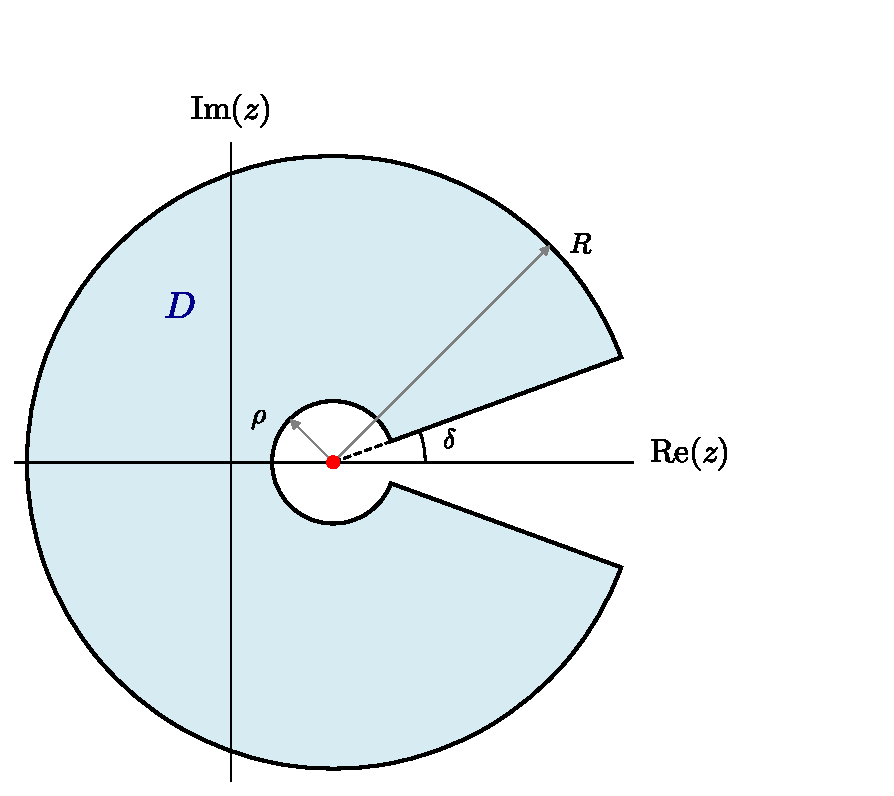
\includegraphics[width=0.6\textwidth]{dominio_D.pdf}
    \caption{Dominio $D$ en el plano complejo.}
    \label{fig:dominio_D}
\end{figure}

Para probar la analiticidad de $I(z)$, basta demostrar que la integral converge uniformemente con respecto a $z$ en el dominio $D$. Esto se sigue inmediatamente de la estimación
\[
\left| t^{b-1}(1-t)^{c-b-1}(1-zt)^{-a} \right| \le M t^{\Re(b)-1} (1-t)^{\Re(c-b)-1},
\]
donde $M$ es el máximo valor de la función continua $|(1-zt)^{-a}|$ para $t \in [0, 1]$ y $z \in D$. La integral
\[
M \int_0^1 t^{\Re(b)-1} (1-t)^{\Re(c-b)-1} \, dt
\]
es convergente bajo las condiciones $\Re(c) > \Re(b) > 0$ y, por tanto, la función integral $I(z)$ es analítica en todo el dominio $D_I = \mathbb{C} \setminus [1, \infty)$ bajo esas condiciones.

Por definición, $I(z)$ es una prolongación analítica de la función hipergeométrica a la región $D_I$. El siguiente paso es demostrar que esta prolongación no es solo una opción, sino que es la única posible. Para ello, nos basamos en el principio de prolongación analítica.

\begin{theorem}[Principio de prolongación analítica]
\label{teo:ppa}
Sean $\Omega$ una región de $\mathbb{C}$ y $f: \Omega \to \mathbb{C}$ una función analítica en $\Omega$. Entonces $f \equiv 0$ en $\Omega$ si y solo si $f = 0$ en un subconjunto de $\Omega$ con punto de acumulación en $\Omega$.
\end{theorem}

\begin{theorem}
\label{teo:unicidad_pa}
Si $\Re(c)>\Re(b)>0$ y $|\arg(1-z)|<\pi$, la función $I(z)$ es la única prolongación analítica de la función hipergeométrica a la región $D_I$.
\end{theorem}

\begin{proof}
Suponemos que existe otra función $J(z)$ que también es una prolongación analítica de la función hipergeométrica a la región $D_I$.
Esto implica por definición que $J(z)$ es analítica en $D_I$ y que $J(z) = {}_{2}F_{1}(a,b;c;z)$ para todo $z$ en el disco $D_S = \{z : |z| < 1\}$.
Para demostrar que $I(z)$ y $J(z)$ son la misma función, definimos la función diferencia
\[
h(z) = I(z) - J(z). 
\]
Como tanto $I(z)$ como $J(z)$ son analíticas en $D_I$, su diferencia $h(z)$ también lo es.
Ahora analizamos el comportamiento de $h(z)$ en el subconjunto $D_S \subset D_I$. Dado que ambas funciones coinciden con ${}_{2}F_{1}(a,b;c;z)$ en este disco, tenemos
\[
h(z) = I(z) - J(z) = 0, \quad z \in D_S. 
\]
El conjunto $D_S$ tiene puntos de acumulación en $D_I$ (de hecho, todos los puntos de $D_S$ son puntos de acumulación y pertenecen a $D_I$). Por lo tanto, la función $h(z)$ satisface el principio de prolongación analítica (Teorema \ref{teo:ppa}), y
\[
h(z) \equiv 0 \quad \text{en } D_I.
\]
Esto significa que $I(z) \equiv J(z)$ para todo $z \in D_I$ y, entonces, es la única prolongación analítica. 
\end{proof}

A pesar de que la representación integral de Euler constituye la prolongación analítica única de la serie hipergeométrica al plano cortado $\mathbb{C} \setminus [1, \infty)$, dicha definición se encuentra severamente restringida por las hipótesis paramétricas $\Re(c) > \Re(b) > 0$. No obstante, siguiendo el enfoque de Lebedev \cite[cap.~9]{lebedev}, es posible relajar estas restricciones sobre los parámetros mediante el uso de la relación de recurrencia 
\begin{equation}
\label{eq:recurrencia_gauss}
\begin{split}
    c(c + 1){}_{2}F_{1}(a,b;c;z) &= c(c - a + 1){}_{2}F_{1}(a, b + 1; c + 2; z) \\ 
    &\quad + a(c - (c - b)z){}_{2}F_{1}(a + 1, b + 1; c + 2; z).
\end{split}
\end{equation}
En efecto, el coeficiente de $z^k$ en el lado derecho de \eqref{eq:recurrencia_gauss} es
\begin{align*}
    & c(c - a + 1)\frac{(a)_k(b + 1)_k}{(c + 2)_k k!} + ac\frac{(a + 1)_k(b + 1)_k}{(c + 2)_k k!} - a(c - b)\frac{(a + 1)_{k-1}(b + 1)_{k-1}}{(c + 2)_{k-1}(k - 1)!} \\
    &\quad = \frac{(a)_k(b)_k}{(c + 2)_k k!} \bigg( c(c - a + 1)\frac{b + k}{b} + c(a + k)\frac{b + k}{b} - (c - b)\frac{(c + k + 1)k}{b} \bigg) \\
    &\quad = (c + k)(c + k + 1)\frac{(a)_k(b)_k}{(c + 2)_k k!} = c(c + 1)\frac{(a)_k(b)_k}{(c)_k k!},
\end{align*}
que coincide con el lado izquierdo. Aplicando esta identidad repetidas veces, podemos representar la función hipergeométrica como la suma
\begin{equation}
\label{eq:recurrencia_gauss_p}
    {}_{2}F_{1}(a,b;c;z) = \sum_{s=0}^p a_{sp}(a,b;c;z){}_{2}F_{1}(a+s,b+p;c+2p;z),
\end{equation}
donde $p$ es un entero positivo y $a_{sp}(a,b;c;z)$ son polinomios en $z$. 

Luego, si los parámetros originales $b$ y $c$ no cumplen las condiciones de Euler, basta con escoger un valor de $p$ suficientemente grande tal que se verifiquen simultáneamente las desigualdades $\Re(b) > -p$ y $\Re(c-b) > -p$. Esto permite el uso de la representación integral en cada una de las funciones ${}_{2}F_{1}(a+s,b+p;c+2p;z)$ del lado derecho de \eqref{eq:recurrencia_gauss_p}, obteniendo así la extensión analítica de la función original para $a$, $b \in \mathbb{C}$ y $c \in \mathbb{C} \setminus \{0,-1,-2,\dots\}$.

Ahora vamos a demostrar que bajo las hipótesis $\Re(c - a - b) > 0$ y $\Re(c) > \Re(b) > 0$, entonces
\begin{equation*}
    {}_{2}F_{1}(a, b; c; 1) = \frac{\Gamma(c)\Gamma(c - a - b)}{\Gamma(c - a)\Gamma(c - b)}.
\end{equation*}
Recordemos que, por el Teorema \ref{teo:convergencia_frontera}, si $\Re(c-a-b)>0$, la serie hipergeométrica es convergente en $z=1$. Bajo estas condiciones, por el teorema de Abel sabemos que ${}_{2}F_{1}(a, b; c; 1) = \lim_{z \to 1^{-}} {}_{2}F_{1}(a, b; c; z)$ y podemos utilizar la representación integral y tomar el límite directamente
\[
{}_{2}F_{1}(a, b; c; 1) = \frac{\Gamma(c)}{\Gamma(b)\Gamma(c - b)} \lim_{z \to 1^{-}} \int_0^1 t^{b-1}(1 - t)^{c - b - 1}(1 - zt)^{-a} \, dt.
\]
El paso del límite bajo el signo integral está justificado por el teorema de la convergencia dominada ya que para $z \in (0,1)$ y $t \in (0,1)$, el módulo del integrando está dominado por la función $t^{\Re(b)-1}(1 - t)^{\Re(c - a - b) - 1}$, la cual es integrable ya que $\Re(c - a - b) > 0$ y $\Re(b)>0$, tenemos entonces
\[
    {}_{2}F_{1}(a, b; c; 1) = \frac{\Gamma(c)}{\Gamma(b)\Gamma(c - b)} \int_0^1 t^{b-1}(1 - t)^{c - a - b - 1} \, dt.
\]
Reconocemos esta integral como la función beta, $B(b, c - a - b)$, que evaluamos en términos de la función Gamma y concluimos
\begin{equation}
    \label{eq:gauss_1}
        {}_{2}F_{1}(a, b; c; 1) =
        \frac{\Gamma(c)}{\Gamma(b)\Gamma(c - b)} \frac{\Gamma(b)\Gamma(c - a - b)}{\Gamma(c - a)} 
        = \frac{\Gamma(c)\Gamma(c - a - b)}{\Gamma(c - a)\Gamma(c - b)}.
\end{equation}

Podemos extender la validez de este resultado eliminando la restricción $\Re(c) > \Re(b) > 0$. Para ello, supongamos inicialmente que los parámetros satisfacen las desigualdades $\Re(c - b) > -1$ y $\Re(b) > -1$.
Bajo estas condiciones, los términos del lado derecho de la relación de recurrencia \eqref{eq:recurrencia_gauss},
\[
    {}_{2}F_{1}(a, b + 1; c + 2; 1) \quad \text{y} \quad {}_{2}F_{1}(a + 1, b + 1; c + 2; 1),
\]
cumplen las restricciones $\Re(c+2) > \Re(b+1) > 0$ necesarias para aplicar el resultado anterior. Entonces podemos usar \eqref{eq:recurrencia_gauss} para afirmar
\begin{align*}
    {}_{2}F_{1}(a, b; c; 1) &= \frac{c - a + 1}{c + 1} \frac{\Gamma(c + 2)\Gamma(c - a - b + 1)}{\Gamma(c - a + 2)\Gamma(c - b + 1)} 
    + \frac{ab}{c(c + 1)} \frac{\Gamma(c + 2)\Gamma(c - a - b)}{\Gamma(c - a + 1)\Gamma(c - b + 1)}
    \\ &=\frac{\Gamma(c)\Gamma(c - a - b)}{\Gamma(c - a)\Gamma(c - b)}.
\end{align*}
Repitiendo este argumento por inducción, podemos relajar las condiciones sobre $b$ y $c$ arbitrariamente. Suponemos que \eqref{eq:gauss_1} se cumple para las condiciones $\Re(c - b) > -n$ y $\Re(b) > -n$ para algún $n \in \mathbb{N}$. Nuevamente, usando la fórmula de recurrencia \eqref{eq:recurrencia_gauss} vemos que los términos del lado derecho de la relación cumplen las restricciones $\Re(c+2) > \Re(b+1) > -n$, luego podemos aplicar el resultado \eqref{eq:gauss_1} bajo las condiciones $\Re(c - b) > -(n+1)$ y $\Re(b) > -(n+1)$. Por lo tanto, la fórmula es válida siempre que se cumpla la condición de convergencia fundamental $\Re(c - a - b) > 0$.
Luego hemos probado el siguiente resultado.
\begin{theorem}[Teorema hipergeométrico de Gauss]
\label{teo:gauss_z1}
Si se cumple la condición $\Re(c - a - b) > 0$, entonces
\[
{}_{2}F_{1}(a, b; c; 1) = \frac{\Gamma(c)\Gamma(c - a - b)}{\Gamma(c - a)\Gamma(c - b)}.
\]
\end{theorem}

Como hemos indicado al principio del capítulo, cuando el parámetro $a$ toma el valor de un entero negativo $a=-n$, la serie hipergeométrica se trunca y se convierte en un polinomio. En este contexto, la aplicación del teorema de Gauss hace aparecer la siguiente identidad fundamental.

\begin{corollary}[Identidad de Chu-Vandermonde]
\label{cor:chu_vandermonde}
Para todo entero no negativo $n$ se verifica que
\[
    {}_{2}F_{1}(-n, b; c; 1) = \frac{(c-b)_n}{(c)_n}.
\]
\end{corollary}

\begin{proof}
Aplicamos el teorema de Gauss con $a = -n$. La condición de convergencia desaparece porque, al tratarse de un polinomio que es una función entera, la identidad es válida siempre. Sustituyendo en la fórmula de Gauss obtenemos
\[
{}_{2}F_{1}(-n, b; c; 1) = \frac{\Gamma(c)\Gamma(c + n - b)}{\Gamma(c + n)\Gamma(c - b)} = \frac{(c-b)_n}{(c)_n}.
\qedhere
\]
\end{proof}

Esta forma compacta de la identidad de Chu-Vandermonde encierra en realidad una de las relaciones más conocidas de la combinatoria clásica. Para desvelarla, necesitamos establecer un puente entre los coeficientes binomiales y el símbolo de Pochhammer.

Utilizando la identidad de reflexión $(x)_n = (-1)^n (1-x-n)_n$ tanto en el numerador como en el denominador del lado derecho del Corolario \ref{cor:chu_vandermonde}, obtenemos la siguiente forma equivalente
\[
{}_{2}F_{1}(-n, b; c; 1) = \frac{(1-c+b-n)_n}{(1-c-n)_n}.
\]
Realizamos el cambio de parámetros $b=-m$ y $c=r-n+1$, donde $m$ y $r$ son números reales, en la expresión anterior y llegamos a que
\begin{equation}
\label{eq:chu-v}
    {}_{2}F_{1}(-n, -m; r-n+1; 1) = \frac{(-m-r)_n}{(-r)_n}.
\end{equation}
Expandiendo el lado derecho vemos que
\begin{align*}
    \binom{r}{n}\frac{(-m-r)_n}{(-r)_n}
    &= \binom{r}{n}\frac{(-1)^n(-m-r)_n}{(-1)^n(-r)_n}\\
    &= \binom{r}{n}\frac{(m+r)(m+r-1)\cdots(m+r-n+1)}{r(r-1)\cdots(r-n+1)} \\
    &= \binom{r}{n}\frac{(m+r)!(r-n)!n!}{r!(m+r-n)!n!} = \binom{m+r}{n}.
\end{align*}
De las identidades
\[
    \frac{(-1)^k(-m)_k}{k!} = \binom{m}{k},
\]
y
\[
    \binom{r}{n}\frac{(-1)^k(-n)_k}{(r-n+1)_k} = \binom{r}{n}\frac{n!(r-n)!}{(n-k)!(r-n+k)!} = \binom{r}{n-k},
\]
para el lado izquierdo de \eqref{eq:chu-v} obtenemos
\begin{align*}
    \binom{r}{n}{}_{2}F_{1}(-n, -m; r-n+1; 1) &= \binom{r}{n}\sum_{k=0}^{n}\frac{(-n)_k(-m)_k}{(r-n+1)_k}\frac{1^k}{k!}\\
    &= \sum_{k=0}^{n}\frac{(-1)^k(-m)_k}{k!}\binom{r}{n}\frac{(-1)^k(-n)_k}{(r-n+1)_k}\\
    &= \sum_{k=0}^{n}\binom{m}{k}\binom{r}{n-k}.
\end{align*}
Finalmente sustituyendo en \eqref{eq:chu-v} llegamos a la conocida identidad combinatoria de Vandermonde\footnote{Esta identidad admite una demostración clásica más directa utilizando funciones generatrices. Partiendo de la igualdad algebraica $(1+x)^m (1+x)^r = (1+x)^{m+r}$ y desarrollando ambos lados mediante el binomio de Newton, el resultado se sigue inmediatamente al igualar el coeficiente de $x^n$ en la expansión derecha $\binom{m+r}{n}$ con el correspondiente en la izquierda, obtenido al aplicar el producto de Cauchy de dos series, el cual es $\sum_{k=0}^n \binom{m}{k}\binom{r}{n-k}$.}
\[
\binom{m+r}{n}=\sum_{k=0}^{n}\binom{m}{k}\binom{r}{n-k}.
\]

\section{Transformaciones lineales}

Las transformaciones de la función hipergeométrica son identidades fundamentales que permiten relacionar la función evaluada en $z$ con la función evaluada en otros puntos relacionados, como $z/(z-1)$, y modificar sus parámetros. Estas transformaciones son una consecuencia directa de la estructura analítica de la función y pueden deducirse elegantemente a partir de la representación integral.

\begin{theorem}[Transformación de Pfaff]
\label{teo:pfaff}
Si $|\arg(1-z)|<\pi$, entonces
\[
{}_{2}F_{1}(a, b; c; z) = (1-z)^{-a} {}_{2}F_{1}\left(a, c-b; c; \frac{z}{z-1}\right).
\]
\end{theorem}

\begin{proof}
Llamamos $I$ a la representación integral de Euler y haciendo el cambio $1-t=s$, se sigue que
\begin{align*}
    I &= \frac{\Gamma(c)}{\Gamma(b)\Gamma(c-b)} \int_0^1 t^{b-1} (1-t)^{c-b-1} (1-zt)^{-a} \, dt \\ &=
    \frac{\Gamma(c)}{\Gamma(b)\Gamma(c-b)} \int_0^1 (1-s)^{b-1} s^{c-b-1} (1-z(1-s))^{-a} \, ds.
\end{align*}
Manipulando el término $(1-z(1-s))$ es fácil ver que
\[ 
1-z(1-s)  = (1-z) \left( 1 - \frac{z}{z-1}s \right), 
\]
y sustituyendo en la integral tenemos
\begin{align*}
    I &= 
    \frac{\Gamma(c)}{\Gamma(b)\Gamma(c-b)} \int_0^1 (1-s)^{b-1} s^{c-b-1} \left((1-z)\left(1-\frac{z}{z-1}s\right)\right)^{-a} \, ds \\ &=
    (1-z)^{-a}\frac{\Gamma(c)}{\Gamma(b)\Gamma(c-b)} \int_0^1 s^{c-b-1}(1-s)^{b-1}  \left(1-\frac{z}{z-1}s\right)^{-a} \, ds \\ &=
    (1-z)^{-a} {}_{2}F_{1}\left(a, c-b; c; \frac{z}{z-1}\right).
    \qedhere
\end{align*}
\end{proof}

Cabe destacar que aunque la demostración se ha construido utilizando la representación integral de Euler, la cual exige que $\Re(c) > \Re(b) > 0$, la identidad final es válida para cualquier valor de los parámetros donde la función hipergeométrica esté definida ($c \neq 0, -1, -2, \dots$), puesto que ambos lados de la igualdad son funciones analíticas respecto a los parámetros $b$ y $c$, el principio de prolongación analítica garantiza que la identidad, al ser válida en el dominio abierto $\Re(c) > \Re(b) > 0$, se extiende de manera única a todo el espacio de parámetros permitido.

Como una de las propiedades de la función hipergeométrica es que es simétrica respecto de los parámetros $a$ y $b$, podemos afirmar que 
\[
    {}_{2}F_{1}(a, b; c; z) = (1-z)^{-b} {}_{2}F_{1}\left(c-a, b; c; \frac{z}{z-1}\right).
\]

A partir de la transformación de Pfaff, podemos deducir otra identidad crucial conocida como la transformación de Euler.

\begin{theorem}[Transformación de Euler]
\label{teo:euler}
Si $|\arg(1-z)|<\pi$, entonces
\[
{}_{2}F_{1}(a, b; c; z) = (1-z)^{c-a-b} {}_{2}F_{1}(c-a, c-b; c; z).
\]
\end{theorem}

\begin{proof}
Haciendo uso de la propiedad de simetría de la función hipergeométrica, aplicamos la transformación de Pfaff sobre el parámetro $a$ y obtenemos
\begin{equation*}
{}_{2}F_{1}(a, b; c; z) = (1-z)^{-b} {}_{2}F_{1}\left(c-a, b; c; \frac{z}{z-1}\right).
\end{equation*}
Ahora, aplicamos nuevamente la transformación de Pfaff a la función hipergeométrica del lado derecho, pero esta vez sobre el parámetro $b$
\begin{align*}
    &(1-z)^{-b}{}_{2}F_{1}\left(c-a, b; c; \frac{z}{z-1}\right) \\ 
    &\quad = (1-z)^{-b}\left(1-\frac{z}{z-1}\right)^{-(c-a)} {}_{2}F_{1}\left(c-a, c-b; c; \frac{\frac{z}{z-1}}{\frac{z}{z-1}-1}\right) \\ 
    &\quad = (1-z)^{c-a-b} {}_{2}F_{1}(c-a, c-b; c; z).
    \qedhere
\end{align*}
\end{proof}

\section{Identidades en valores especiales}

La representación integral de Euler no solo nos permite extender el dominio de la función, sino que también es una herramienta poderosa para deducir el valor de la función hipergeométrica en puntos específicos del plano complejo, mediante cambios de variable adecuados en la integral. A continuación, demostramos dos identidades clásicas.

\begin{theorem}[Teorema de Kummer]
\label{teo:kummer_z_minus_1}
Si $\Re(b) > 0$ y $\Re(a)< 1$, entonces
\[
{}_{2}F_{1}(a, b; 1-a+b; -1) = \frac{\Gamma(1-a+b) \Gamma(1+\frac{b}{2})}{\Gamma(1+\frac{b}{2}-a) \Gamma(1+b)}.
\]
\end{theorem}

\begin{proof}
Partimos de la representación integral de Euler evaluada en $z=-1$ con $c=1-a+b$. Si denotamos por $I$ la integral para ${}_{2}F_{1}(a,b;1-a+b;-1)$, tenemos
\begin{align*}
 I &= 
 \frac{\Gamma(1-a+b)}{\Gamma(b)\Gamma(1-a)} \int_0^1 t^{b-1} (1-t)^{-a} (1+t)^{-a} \, dt \\ &= 
 \frac{\Gamma(1-a+b)}{\Gamma(b)\Gamma(1-a)}\int_0^1 t^{b-1} (1-t^2)^{-a} \, dt.   
\end{align*}
Realizamos el cambio de variable $t^2 = u$,
\begin{align*}
   I &=   
   \frac{\Gamma(1-a+b)}{2\Gamma(b)\Gamma(1-a)} \int_0^1 u^{\frac{b}{2}-1} (1-u)^{-a} \, du \\ 
   &= \frac{\Gamma(\frac{b}{2})}{2\Gamma(b)} \frac{\Gamma(1-a+b)}{\Gamma(\frac{b}{2}+1-a)}.
\end{align*}
Como
\[ 
\frac{\Gamma(\frac{b}{2})}{2\Gamma(b)} = \frac{\Gamma(1+\frac{b}{2})}{\Gamma(1+b)},
\]
concluimos que
\begin{equation*}
  {}_{2}F_{1}(a, b; 1-a+b; -1) = \frac{\Gamma(1-a+b) \Gamma(1+\frac{b}{2})}{\Gamma(1+\frac{b}{2}-a) \Gamma(1+b)}.
\qedhere  
\end{equation*}
\end{proof}

\begin{theorem}[Identidad de Bailey]
\label{teo:bailey}
Si $\Re(c)>\Re(1-a)>0$, entonces
\[
{}_{2}F_{1}\left(a, 1-a; c; \frac{1}{2}\right) = \frac{\Gamma(\frac{c}{2})\Gamma(\frac{c+1}{2})}{\Gamma(\frac{c+a}{2})\Gamma(\frac{c-a+1}{2})}.
\]
\end{theorem}

\begin{proof}
Partimos nuevamente de la representación integral con $z=1/2$ y $b=1-a$ y llamamos $I$ a ${}_{2}F_{1}(a,1-a;c;1/2)$. De este modo
\begin{align*}
   I &= 
   \frac{\Gamma(c)}{\Gamma(1-a)\Gamma(c+a-1)} \int_0^1 t^{-a} (1-t)^{c+a-2} \left(1-\frac{t}{2}\right)^{-a} \, dt \\ 
   &= \frac{2^a \Gamma(c)}{\Gamma(1-a)\Gamma(c+a-1)}\int_0^1 t^{-a} (1-t)^{c+a-2} (2-t)^{-a} \, dt.
\end{align*}
Realizamos, sucesivamente, los cambios de variable $1 - t = u$ y $u^2 = v$ para tener que 
\begin{align*}
   I &= 
   \frac{2^a \Gamma(c)}{\Gamma(1-a)\Gamma(c+a-1)} \int_0^1 (1-u)^{-a} u^{c+a-2} (1+u)^{-a} \, du \\ 
   &= \frac{2^a \Gamma(c)}{\Gamma(1-a)\Gamma(c+a-1)} \int_0^1 u^{c+a-2} (1-u^2)^{-a} \, du \\
   &= \frac{2^{a-1} \Gamma(c)}{\Gamma(1-a)\Gamma(c+a-1)} \int_0^1 v^{\frac{c+a-3}{2}} (1-v)^{-a} \, dv \\ 
   &= \frac{ 2^{a-1}\Gamma(c)}{\Gamma(1-a)\Gamma(c+a-1)} \frac{\Gamma(\frac{c+a-1}{2})\Gamma(1-a)}{\Gamma(\frac{c-a+1}{2})}.
\end{align*}
La fórmula de duplicación de Legendre nos dice que $\Gamma(z)\Gamma(z+1/2) = 2^{1-2z}\sqrt{\pi}\Gamma(2z)$, y aplicándola al término $\Gamma(c+a-1)$ obtenemos
\[ 
I = \frac{2^{a-1}\Gamma(c)\Gamma(\frac{c+a-1}{2})}{2^{c+a-2} \pi^{-1/2} \Gamma(\frac{c+a-1}{2})\Gamma(\frac{c+a}{2})\Gamma(\frac{c-a+1}{2})} = \frac{\sqrt{\pi} 2^{1-c} \Gamma(c)}{\Gamma(\frac{c+a}{2})\Gamma(\frac{c-a+1}{2})}.
\]
De forma análoga aplicamos la fórmula de duplicación a $\Gamma(c)$ y concluimos
\[ 
{}_{2}F_{1}\left(a, 1-a; c; \frac{1}{2}\right) = \frac{\Gamma(\frac{c}{2})\Gamma(\frac{c+1}{2})}{\Gamma(\frac{c+a}{2})\Gamma(\frac{c-a+1}{2})}.
\qedhere
\]
\end{proof}

Otro resultado interesante es el segundo teorema de suma de Gauss, que evalúa la serie en $z=1/2$ bajo condiciones específicas de los parámetros. La demostración está tomada de \cite{choi2007}.

\begin{theorem}[Segundo teorema hipergeométrico de Gauss]
\label{teo:gauss_segundo}
Si $\Re(b) > 0$ y $\Re(a-b+1) > 0$, entonces
\[
{}_{2}F_{1}\left(a, b; \frac{a+b+1}{2}; \frac{1}{2}\right) = \frac{\sqrt{\pi} \Gamma(\frac{a+b+1}{2})}{\Gamma(\frac{a+1}{2})\Gamma(\frac{b+1}{2})}.
\]
\end{theorem}

\begin{proof}
Comenzamos obteniendo una representación integral trigonométrica para ${}_{2}F_{1}(a,b;c;1/2)$ con $c$ arbitrario. Tenemos
\begin{align*}
  {}_{2}F_{1}(a,b;c;1/2) &=  
  \frac{\Gamma(c)}{\Gamma(b)\Gamma(c-b)} \int_0^1 t^{b-1} (1-t)^{c-b-1} \left(1-\frac{t}{2}\right)^{-a} \, dt \\ 
  &= \frac{2^a\Gamma(c)}{\Gamma(b)\Gamma(c-b)} \int_0^1 t^{b-1} (1-t)^{c-b-1} (2-t)^{-a} \, dt
\end{align*}
y realizando el cambio de variable $t = 1 - \tan^2(\theta/2)$ la integral nos queda
\begin{align*}
    &\int_0^{\pi/2} \left( \frac{\cos\theta}{\cos^2(\theta/2)} \right)^{b-1}(\tan(\theta/2))^{2(c-b-1)}(\sec(\theta/2))^{-2a} \frac{\sin(\theta/2)}{\cos^3(\theta/2)} \, d\theta \\ 
    &= \int_0^{\pi/2} (\cos\theta)^{b-1} (\sin(\theta/2))^{2c-2b-1} (\cos(\theta/2))^{2a-2c+1} \, d\theta.
\end{align*}
Finalmente, obtenemos la expresión integral deseada para  ${}_{2}F_{1}(a,b;c;1/2)$
\begin{equation}
\label{exp_1/2}
  {}_{2}F_{1}(a,b;c;1/2) = \frac{2^a\Gamma(c)}{\Gamma(b)\Gamma(c-b)} \int_0^{\pi/2} (\cos\theta)^{b-1} \left(\sin\frac{\theta}{2}\right)^{2c-2b-1} \left(\cos\frac{\theta}{2}\right)^{2a-2c+1} \, d\theta.  
\end{equation}
Tomando $c = (a+b+1)/2$ en \eqref{exp_1/2}, se llega a que
\begin{align*}
    {}_{2}F_{1}\left(a, b; \frac{a+b+1}{2}; \frac{1}{2}\right) &= \frac{2^a\Gamma(\frac{a+b+1}{2})}{\Gamma(b)\Gamma(\frac{a-b+1}{2})} \int_0^{\pi/2} (\cos\theta)^{b-1} \left(\sin\frac{\theta}{2}\right)^{a-b} \left(\cos\frac{\theta}{2}\right)^{a-b} \, d\theta \\
    &= \frac{2^a\Gamma(\frac{a+b+1}{2})}{2^{a-b}\Gamma(b)\Gamma(\frac{a-b+1}{2})} \int_0^{\pi/2} (\cos\theta)^{b-1} (\sin\theta)^{a-b} \, d\theta \\
    &= \frac{2^{b-1}\Gamma(\frac{a+b+1}{2})}{\Gamma(b)\Gamma(\frac{a-b+1}{2})} \frac{\Gamma(\frac{b}{2})\Gamma(\frac{a-b+1}{2})}{\Gamma(\frac{a+1}{2})} \\
    &= \frac{2^{b-1}\Gamma(\frac{a+b+1}{2})\Gamma(\frac{b}{2})}{\Gamma(b)\Gamma(\frac{a+1}{2})}.
\end{align*}
Usamos la fórmula de duplicación de Legendre con $z = b/2$ para deducir que
\[
\Gamma\left(\frac{b}{2}\right)\Gamma\left(\frac{b+1}{2}\right) = 2^{1-b}\sqrt{\pi}\Gamma(b),
\]
y obtenemos finalmente el segundo teorema hipergeométrico de Gauss
\[ 
{}_{2}F_{1}\left(a, b; \frac{a+b+1}{2}; \frac{1}{2}\right) = \frac{\sqrt{\pi} \Gamma(\frac{a+b+1}{2})}{\Gamma(\frac{a+1}{2})\Gamma(\frac{b+1}{2})}.
\qedhere
\]
\end{proof}

La versatilidad de la representación integral y de las transformaciones lineales permite obtener evaluaciones exactas no solo en la frontera del disco de convergencia o en $z=1/2$, sino también en otros valores racionales del interior del disco. Un ejemplo notable es la identidad en $z=1/4$ atribuida a Gosper y cuya demostración hemos tomado de \cite{hakimoglu2026gosper}.

\begin{theorem}[Fórmula de Gosper]
\label{teo:gosper}
Si $\Re(b) > 0$ y $5/2 - 2b \notin \{0, -1, -2, \dots\}$, se verifica
\[
{}_{2}F_{1}\left(\frac{1}{2}, b; \frac{5}{2}-2b; \frac{1}{4}\right) = \frac{2^{2b}\sqrt{\pi}}{3}\frac{\Gamma(\frac{5}{2}-2b)}{\Gamma^{2}(\frac{3}{2}-b)}.
\]
\end{theorem}

\begin{proof}
Comenzamos aplicando la transformación de Euler (Teorema \ref{teo:euler}) a la función hipergeométrica original con $a=1/2$, $c=5/2-2b$ y $z=1/4$,
\begin{align*}
    {}_{2}F_{1}\left(\frac{1}{2}, b; \frac{5}{2}-2b; \frac{1}{4}\right) &= \left(1-\frac{1}{4}\right)^{\left(\frac{5}{2}-2b\right)-\frac{1}{2}-b} {}_{2}F_{1}\left(2-2b, \frac{5}{2}-3b; \frac{5}{2}-2b; \frac{1}{4}\right) \\
    &= \left(\frac{3}{4}\right)^{2-3b} {}_{2}F_{1}\left(2-2b, \frac{5}{2}-3b; \frac{5}{2}-2b; \frac{1}{4}\right).
\end{align*}
Si aplicamos la representación integral de Euler y denotamos la integral resultante como $I$ vemos que
\[
    I = \frac{\Gamma(\frac{5}{2}-2b)}{\Gamma(\frac{5}{2}-3b)\Gamma(b)} \int_{0}^{1} t^{\frac{3}{2}-3b} (1-t)^{b-1} \left(1-\frac{t}{4}\right)^{2b-2} \, dt.
\]
Utilizamos el cambio de variable $t = 4u/(1+u)^2$ y obtenemos
\begin{align*}
     I &= \frac{\Gamma(\frac{5}{2}-2b)}{\Gamma(\frac{5}{2}-3b)\Gamma(b)} 4^{\frac{5}{2}-3b} \int_{0}^{1} u^{\frac{3}{2}-3b} (1-u)^{2b-1} (1+u+u^2)^{2b-2} \, du \\
     &= \frac{\Gamma(\frac{5}{2}-2b)}{\Gamma(\frac{5}{2}-3b)\Gamma(b)} 4^{\frac{5}{2}-3b} \int_{0}^{1} u^{\frac{3}{2}-3b} (1-u) (1-u^3)^{2b-2} \, du \\
     &= \frac{\Gamma(\frac{5}{2}-2b)}{\Gamma(\frac{5}{2}-3b)\Gamma(b)} 4^{\frac{5}{2}-3b} \int_{0}^{1} \left(u^{\frac{3}{2}-3b} - u^{\frac{5}{2}-3b}\right) (1-u^3)^{2b-2} \, du.
\end{align*}
Con el cambio $u^3 = v$ obtenemos
\begin{align*}
    I &= \frac{\Gamma(\frac{5}{2}-2b)}{3\Gamma(\frac{5}{2}-3b)\Gamma(b)} 4^{\frac{5}{2}-3b} \int_{0}^{1} \left(v^{\frac{5}{6}-b-1} - v^{\frac{7}{6}-b-1}\right) (1-v)^{2b-2} \, dv \\
    &= \frac{\Gamma(\frac{5}{2}-2b)}{3\Gamma(\frac{5}{2}-3b)\Gamma(b)} 4^{\frac{5}{2}-3b} \left( B\left(\frac{5}{6}-b, 2b-1\right) - B\left(\frac{7}{6}-b, 2b-1\right) \right).
\end{align*}
Denotamos como $\Delta$ a la diferencia de funciones Beta 
\begin{align*}
    \Delta &=  B\left(\frac{5}{6}-b, 2b-1\right) - B\left(\frac{7}{6}-b, 2b-1\right)\\
    &= \Gamma(2b-1) \left( \frac{\Gamma\left(\frac{5}{6}-b\right)}{\Gamma\left(b-\frac{1}{6}\right)} - \frac{\Gamma\left(\frac{7}{6}-b\right)}{\Gamma\left(b+\frac{1}{6}\right)} \right).
\end{align*}
Por la fórmula de reflexión de Euler podemos observar que
\[
    \frac{1}{\Gamma\left(b-\frac{1}{6}\right)} = \frac{\Gamma\left(\frac{7}{6}-b\right) \sin\left(\pi\left(b-\frac{1}{6}\right)\right)}{\pi},
\]
y
\[
    \frac{1}{\Gamma\left(b+\frac{1}{6}\right)} = \frac{\Gamma\left(\frac{5}{6}-b\right) \sin\left(\pi\left(b+\frac{1}{6}\right)\right)}{\pi}.
\]
Sustituyendo estas expresiones en $\Delta$, obtenemos
\begin{align*}
        \Delta &= \frac{\Gamma(2b-1)\Gamma\left(\frac{5}{6}-b\right)\Gamma\left(\frac{7}{6}-b\right)}{\pi} \left( \sin\left(\pi b - \frac{\pi}{6}\right) - \sin\left(\pi b + \frac{\pi}{6}\right) \right) \\
        &= -\frac{\Gamma(2b-1)\Gamma\left(\frac{5}{6}-b\right)\Gamma\left(\frac{7}{6}-b\right) \cos(\pi b)}{\pi}.
\end{align*}
Por tanto, vemos que
\begin{align*}
    {}_{2}F_{1}\left(\frac{1}{2}, b; \frac{5}{2}-2b; \frac{1}{4}\right)
    &\quad = \left(\frac{3}{4}\right)^{2-3b} \frac{\Gamma\left(\frac{5}{2}-2b\right)}{3\Gamma\left(\frac{5}{2}-3b\right)\Gamma(b)} 4^{\frac{5}{2}-3b} \Delta \\
    &\quad = \frac{2 \cdot 3^{1-3b} \Gamma\left(\frac{5}{2}-2b\right)}{\Gamma\left(\frac{5}{2}-3b\right)\Gamma(b)} \Delta \\
    &\quad = -\frac{2 \cdot 3^{1-3b} \Gamma\left(\frac{5}{2}-2b\right) \Gamma(2b-1) \Gamma\left(\frac{5}{6}-b\right)\Gamma\left(\frac{7}{6}-b\right) \cos(\pi b)}{\pi \Gamma\left(\frac{5}{2}-3b\right)\Gamma(b)}.
\end{align*}
En este punto, interviene el teorema de multiplicación de Gauss-Legendre.\footnote{Este teorema generaliza las fórmulas de duplicación ($m=2$) y triplicación ($m=3$), estableciendo que para todo entero positivo $m$ se verifica la identidad 
\[
\prod_{k=0}^{m-1} \Gamma\left(z + \frac{k}{m}\right) = (2\pi)^{\frac{m-1}{2}} m^{\frac{1}{2} - mz} \Gamma(mz).
\]
} Para el caso de triplicación ($m=3$) evaluado en $z = 5/6 - b$, tenemos que 
\[
\Gamma\left(\frac{5}{2}-3b\right) = \frac{3^{2-3b}}{2\pi} \Gamma\left(\frac{5}{6}-b\right)\Gamma\left(\frac{7}{6}-b\right)\Gamma\left(\frac{3}{2}-b\right).
\]
Simplificando,
\begin{align*}
    & {}_{2}F_{1}\left(\frac{1}{2}, b; \frac{5}{2}-2b; \frac{1}{4}\right) \\
    &\quad = -\frac{2 \cdot 3^{1-3b} \Gamma\left(\frac{5}{2}-2b\right) \Gamma(2b-1) \cos(\pi b)}{\pi \Gamma(b)}  \frac{2\pi}{3^{2-3b} \Gamma\left(\frac{3}{2}-b\right)}  \\
    &\quad = -\frac{4}{3} \frac{\Gamma\left(\frac{5}{2}-2b\right)\Gamma(2b-1)\cos(\pi b)}{\Gamma(b)\Gamma\left(\frac{3}{2}-b\right)}.
\end{align*}
Utilizando la fórmula de duplicación de Legendre sobre $\Gamma(2b-1)$ se sigue que
\begin{align*}
    {}_{2}F_{1}\left(\frac{1}{2}, b; \frac{5}{2}-2b; \frac{1}{4}\right) &= -\frac{4}{3} \frac{\Gamma\left(\frac{5}{2}-2b\right)}{\Gamma(b)\Gamma\left(\frac{3}{2}-b\right)} \frac{2^{2b-2}}{\sqrt{\pi}} \Gamma\left(b-\frac{1}{2}\right)\Gamma(b)  \cos(\pi b) \\
    &= -\frac{2^{2b}}{3\sqrt{\pi}} \frac{\Gamma\left(\frac{5}{2}-2b\right)}{\Gamma\left(\frac{3}{2}-b\right)} \Gamma\left(b-\frac{1}{2}\right) \cos(\pi b).
\end{align*}
Por último, aplicando la fórmula de reflexión sobre los términos restantes se tiene que
\[
\Gamma\left(b-\frac{1}{2}\right)\Gamma\left(\frac{3}{2}-b\right) = \frac{\pi}{\sin\left(\pi\left(b-\frac{1}{2}\right)\right)} = -\frac{\pi}{\cos(\pi b)},
\]
concluyendo con la evaluación exacta
\[
    {}_{2}F_{1}\left(\frac{1}{2}, b; \frac{5}{2}-2b; \frac{1}{4}\right) = \frac{2^{2b}\sqrt{\pi}}{3} \frac{\Gamma\left(\frac{5}{2}-2b\right)}{\Gamma^{2}\left(\frac{3}{2}-b\right)}. \qedhere
\]
\end{proof}


\chapter[Conexión con polinomios ortogonales]{Conexión de la función hipergeométrica con polinomios ortogonales}

En el capítulo anterior hemos estudiado la función hipergeométrica desde una perspectiva general, tratándola como una serie de potencias infinita que, mediante su continuación analítica, define una función analítica en el plano complejo cortado. Hemos analizado su convergencia, su representación integral y sus propiedades de transformación bajo la suposición de que la serie no se trunca.

Sin embargo, como ya adelantamos en la Sección \ref{sec:definicion_propiedades}, existe una situación de particular importancia cuando la serie hipergeométrica se reduce a un polinomio. Si el parámetro $a$ (o por simetría, el $b$) toma el valor de un entero no positivo $a = -m$, el símbolo de Pochhammer se anula para todo $n \ge m+1$, lo que trunca la serie infinita en una suma finita de grado $m$. 

Este fenómeno de terminación es el fundamento que permite expresar diversas familias de polinomios ortogonales clásicos en términos de la función hipergeométrica. En las siguientes secciones exploraremos cómo los polinomios de Jacobi, y sus casos particulares (Gegenbauer y Legendre), pueden entenderse como casos específicos de esta función hipergeométrica polinómica bajo cambios de variable y parámetros adecuados.

\section{Polinomios de Jacobi}
\label{sec:polinomios_jacobi}

Los polinomios de Jacobi, denotados por $P_n^{(\alpha, \beta)}(x)$, constituyen la clase más general de polinomios ortogonales clásicos en un intervalo finito. Muchas otras familias importantes, como los polinomios de Legendre y Gegenbauer, pueden obtenerse como casos particulares de estos eligiendo adecuadamente los parámetros $\alpha$ y $\beta$.

Existen diversas formas de introducir estos polinomios, pero una de las más compactas y útiles para el cálculo es mediante la fórmula de Rodrigues.

\begin{definition}[Fórmula de tipo Rodrigues]
\label{def:rodrigues}
Una fórmula de tipo Rodrigues define el $n$-ésimo polinomio $P_n(x)$ de una familia mediante la expresión
\begin{equation*}
    P_n(x) = \frac{1}{K_n w(x)} \frac{d^n}{dx^n} \left( w(x) q(x)^n \right),
\end{equation*}
donde $w(x)$ es una función peso, $q(x)$ es un polinomio independiente de $n$, y $K_n$ es una constante de normalización.
\end{definition}

\begin{definition}[Polinomios de Jacobi]
\label{def:jacobi_rodrigues}
Para $n \in \mathbb{N} \cup \{0\}$ y parámetros reales $\alpha, \beta > -1$, el polinomio de Jacobi de grado $n$, $P_n^{(\alpha, \beta)}(x)$, se define mediante la fórmula de tipo Rodrigues
\begin{equation*}
    P_n^{(\alpha, \beta)}(x) = \frac{(-1)^n}{2^n n!} (1-x)^{-\alpha} (1+x)^{-\beta} \frac{d^n}{dx^n} ((1-x)^{\alpha+n} (1+x)^{\beta+n}).
\end{equation*}
\end{definition}

El primer y más obvio paso es probar que los polinomios de Jacobi son, efectivamente, polinomios y de grado $n$.

\begin{prop}
    \label{prop:jacobi_es_polinomio}
$P_n^{(\alpha, \beta)}(x)$ es un polinomio de grado $n$.
\end{prop}
\begin{proof}
Aplicando la regla de Leibniz para la derivada $n$-ésima de un producto al interior del operador en la fórmula de Rodrigues, obtenemos
\[
\frac{d^n}{dx^n} ((1-x)^{\alpha+n} (1+x)^{\beta+n}) = \sum_{k=0}^n \binom{n}{k} \frac{d^k}{dx^k} \left( (1-x)^{\alpha+n} \right) \frac{d^{n-k}}{dx^{n-k}} \left( (1+x)^{\beta+n} \right).
\]
Como
\[
    \frac{d^k}{dx^k} (1-x)^{\alpha+n} =  (-1)^k \frac{\Gamma(\alpha+n+1)}{\Gamma(\alpha+n-k+1)} (1-x)^{\alpha+n-k},
\]
y 
\[
    \frac{d^{n-k}}{dx^{n-k}} (1+x)^{\beta+n} = \frac{\Gamma(\beta+n+1)}{\Gamma(\beta+k+1)} (1+x)^{\beta+k},
\]
sustituyendo en la fórmula de Rodrigues,
\begin{equation}
\label{sum_jacobi}
    P_n^{(\alpha, \beta)}(x) = \frac{(-1)^n}{2^n n!} \sum_{k=0}^n \binom{n}{k} (-1)^k C_{n,k} (1-x)^{n-k} (1+x)^k,
\end{equation}
donde
\[
C_{n,k} = \frac{\Gamma(\alpha+n+1)\Gamma(\beta+n+1)}{\Gamma(\alpha+n-k+1)\Gamma(\beta+k+1)}.
\]
Puesto que cada término de la suma contiene el producto $(1-x)^{n-k}(1+x)^k$, queda demostrado que $P_n^{(\alpha, \beta)}(x)$ es, efectivamente, un polinomio de grado menor o igual que $n$.
Veamos que efectivamente es un polinomio de grado $n$. Puesto que
\[
(1-x)^{n-k} (1+x)^k = (-1)^{n-k} x^n + \text{términos de menor grado},
\]
el coeficiente de $x^n$ será 
\[
\frac{1}{2^n n!}\sum_{k=0}^{n}\binom{n}{k} C_{n,k}
\]
que es estrictamente positivo.\footnote{El valor exacto del coeficiente principal de los polinomios de Jacobi puede verse en el Lema \ref{lema:coeficiente_principal}.}
\end{proof}

Aplicando la expresión explícita obtenida en la demostración anterior, podemos determinar fácilmente el valor del polinomio y su derivada en $x=1$. Este resultado será fundamental más adelante, ya que nos proporcionará la constante de normalización necesaria para establecer la identidad entre los polinomios de Jacobi y la función hipergeométrica.

\begin{prop}
\label{prop:valor_en_1}
En $x=1$ se verifica
\begin{equation*}
    P_n^{(\alpha, \beta)}(1) = \binom{n+\alpha}{n} \quad \text{y} \quad (P_n^{(\alpha, \beta)})'(1) = \frac{n+\alpha+\beta+1}{2} \binom{n+\alpha}{n-1}.
\end{equation*}
\end{prop}

\begin{proof}
Consideramos la expresión explícita obtenida en la demostración de la Proposición~\ref{prop:jacobi_es_polinomio} y evaluamos dicha expresión en $x=1$. Observamos que el factor $(1-x)^{n-k}$ es nulo para todo $k < n$. Por tanto, el único término de la suma que no se anula es el correspondiente al índice $k=n$. Como
\[
C_{n,n} = \frac{\Gamma(\alpha+n+1)}{\Gamma(\alpha+1)},
\]
sustituyendo en la fórmula del polinomio se sigue
\[
P_n^{(\alpha, \beta)}(1) = \frac{(-1)^n}{2^n n!} \left( (-1)^n \frac{\Gamma(\alpha+n+1)}{\Gamma(\alpha+1)} \cdot 2^n \right),
\]
y simplificando obtenemos finalmente
\[
P_n^{(\alpha, \beta)}(1) = \frac{\Gamma(\alpha+n+1)}{n! \, \Gamma(\alpha+1)} = \binom{n+\alpha}{n}.
\]
Para el valor en la derivada, partimos de la fórmula \eqref{sum_jacobi}  y derivamos
\begin{align*}
    (P_n^{(\alpha, \beta)})'(x) &= \frac{(-1)^n}{2^n n!} \sum_{k=0}^n \binom{n}{k} (-1)^k C_{n,k} \big( -(n-k)(1-x)^{n-k-1}(1+x)^k \\
    &\qquad + k(1-x)^{n-k}(1+x)^{k-1} \big).
\end{align*}
Evaluamos en $x=1$ y, puesto que los únicos términos que sobreviven son $n-1$ y $n$, tenemos que
\begin{align*}
    (P_n^{(\alpha, \beta)})'(1) &= \frac{(-1)^n}{2^n n!} \left( \binom{n}{n-1} (-1)^{n-1} C_{n,n-1} ( -2^{n-1} ) + (-1)^n C_{n,n} ( n2^{n-1} ) \right) \\
    &= \frac{1}{2(n-1)!} \left( C_{n,n} + C_{n,n-1} \right).
\end{align*}
Como
\[
C_{n,n-1} = \frac{\Gamma(\alpha+n+1)\Gamma(\beta+n+1)}{\Gamma(\alpha+2)\Gamma(\beta + n)},
\]
se sigue que
\begin{align*}
    C_{n,n} + C_{n,n-1} &= \frac{\Gamma(\alpha+n+1)}{\Gamma(\alpha+1)} \left( \frac{n+\alpha+\beta+1}{\alpha+1} \right)\\ 
    &= \frac{\Gamma(\alpha+n+1)}{\Gamma(\alpha+2)} (n+\alpha+\beta+1).
\end{align*}
Sustituyendo esta suma en la expresión de la derivada, obtenemos finalmente
\begin{equation*}
    (P_n^{(\alpha, \beta)})'(1) = \frac{n+\alpha+\beta+1}{2(n-1)!}  \frac{\Gamma(\alpha+n+1)}{\Gamma(\alpha+2)} = \frac{n+\alpha+\beta+1}{2} \binom{n+\alpha}{n-1}.
    \qedhere
\end{equation*}
\end{proof}

Una de las propiedades fundamentales de los polinomios de Jacobi es que son soluciones de una ecuación diferencial lineal de segundo orden. A continuación, deduciremos dicha ecuación directamente a partir de la fórmula de Rodrigues introducida en la definición anterior.

\begin{theorem}[Ecuación diferencial de Jacobi]
\label{teo:edo_jacobi}
El polinomio de Jacobi $y(x) = P_n^{(\alpha, \beta)}(x)$ satisface la siguiente ecuación diferencial homogénea de segundo orden
\begin{equation*}
    (1-x^2)y'' + (\beta - \alpha - (\alpha + \beta + 2)x)y' + n(n + \alpha + \beta + 1)y = 0.
\end{equation*}
\end{theorem}

\begin{proof}
Para simplificar la notación en el desarrollo, denotaremos por $V_n(x)$ a la parte diferencial de la fórmula de Rodrigues
\[
V_n(x) = \frac{d^n}{dx^n} ((1-x)^{n+\alpha} (1+x)^{n+\beta}).
\]
Definimos la función auxiliar $f(x)$ como el argumento de dicha derivada
\[
f(x) = (1-x)^{n+\alpha} (1+x)^{n+\beta}.
\]
La demostración procede en dos etapas: primero hallaremos la ecuación diferencial que satisface $V_n(x)$ y posteriormente recuperaremos la ecuación para $P_n^{(\alpha, \beta)}(x)$.
Derivamos $f(x)$ una vez con respecto a $x$ y tenemos
\begin{align*}
    f'(x) &=
    -(n+\alpha)(1-x)^{n+\alpha-1}(1+x)^{n+\beta} + (n+\beta)(1-x)^{n+\alpha}(1+x)^{n+\beta-1} \\ 
    &= (1-x)^{n+\alpha-1}(1+x)^{n+\beta-1} \left[ -(n+\alpha)(1+x) + (n+\beta)(1-x) \right] \\ 
    &= (1-x)^{n+\alpha-1}(1+x)^{n+\beta-1} ((\beta - \alpha) - x(2n + \alpha + \beta)).
\end{align*}
Multiplicando ambos lados por $(1-x^2)$ vemos que $f(x)$ satisface la ecuación diferencial de primer orden
\begin{equation}
\label{eq:f_ode_primer_orden}
    (1-x^2)f'(x) = ((\beta - \alpha) - (2n + \alpha + \beta)x)f(x).   
\end{equation}
Ahora aplicamos la regla de Leibniz para derivar la expresión \eqref{eq:f_ode_primer_orden} $n+1$ veces. Para el término de la izquierda $(1-x^2)f'(x)$, al derivar $n+1$ veces, los únicos términos no nulos son
    \[
     (1-x^2)f^{(n+2)}(x) -2(n+1)xf^{(n+1)}(x) - n(n+1)f^{(n)}(x).
    \]
Para el término de la derecha $((\beta - \alpha) - (2n + \alpha + \beta)x)f(x)$, solo sobreviven 
    \[
    ((\beta - \alpha) - (2n + \alpha + \beta)x)f^{(n+1)}(x) - (n+1)(2n + \alpha + \beta)f^{(n)}(x).
    \]
Simplificando, agrupando por orden de derivación, y recordando que $V_n(x) = f^{(n)}(x)$, obtenemos la ecuación diferencial
\[
(1-x^2)V_n''(x) + ((\alpha - \beta) + x(\alpha + \beta - 2))V_n'(x) + (n+1)(n + \alpha + \beta)V_n(x) = 0.
\]
De la fórmula de Rodrigues, sabemos que $P_n^{(\alpha, \beta)}(x)$ y $V_n(x)$ se relacionan mediante la identidad
\[
P_n^{(\alpha, \beta)}(x) = K_n (1-x)^{-\alpha} (1+x)^{-\beta} V_n(x),
\]
donde $K_n$ es una constante. Sea el peso $w(x) = (1-x)^{\alpha} (1+x)^{\beta}$, invirtiendo la relación, escribimos $V_n(x)$ en términos de $y(x) = P_n^{(\alpha, \beta)}(x)$ y tenemos
\[
V_n(x) = \frac{1}{K_n} (1-x)^{\alpha} (1+x)^{\beta} y(x) = \frac{1}{K_n}w(x)y(x).
\]
Calculamos ahora las derivadas necesarias para sustituir en la ecuación diferencial
\[
V_n'(x) =\frac{1}{K_n} (w'(x)y(x) + w(x)y'(x))
\]
y
\[
V_n''(x) =\frac{1}{K_n} (w''(x)y(x) + 2w'(x)y'(x) + w(x)y''(x)).
\]
Luego, tras sustituir, se sigue
\begin{align*}
    &(1-x^2)wy'' + \big( 2(1-x^2)w' + ((\alpha - \beta) + x(\alpha + \beta - 2))w \big)y' \\
    &+ \big( (1-x^2)w'' + ((\alpha - \beta) + x(\alpha + \beta - 2))w' + (n+1)(n + \alpha + \beta)w \big)y = 0, 
\end{align*}
y dividiendo por $w$ obtenemos
\begin{align*}
    &(1-x^2)y'' + \left( \frac{2(1-x^2)w'}{w} + (\alpha - \beta) + x(\alpha + \beta - 2) \right)y' \\
    &+ \bigg( \frac{(1-x^2)w''}{w} + \frac{((\alpha - \beta) + x(\alpha + \beta - 2))w'}{w} + (n+1)(n + \alpha + \beta) \bigg)y = 0.
\end{align*}
De las relaciones
\[
\frac{w'}{w} = \frac{-\alpha}{1-x} + \frac{\beta}{1+x} = \frac{\beta - \alpha - x(\alpha+\beta)}{1-x^2},
\]
y
\[
\left(\frac{w'}{w}\right)' = \frac{w'' \cdot w - w' \cdot w'}{w^2} = \frac{w''}{w} - \left(\frac{w'}{w}\right)^2,
\]
obtenemos la expresión de $w''/w$
\begin{align*}
    \frac{w''}{w} &= -\frac{(\alpha+\beta)(1+x^2) + 2(\alpha-\beta)x}{(1-x^2)^2} + \frac{((\alpha+\beta)x + (\alpha-\beta) )^2}{(1-x^2)^2} \\ 
    &= \frac{((\alpha+\beta)^2 - \alpha-\beta)x^2 + 2(\alpha-\beta)(\alpha+\beta-1)x + ((\alpha-\beta)^2 - \alpha-\beta)}{(1-x^2)^2}.
\end{align*}
Finalmente, sustituyendo y simplificando todo llegamos a la ecuación diferencial de los polinomios de Jacobi
\[
     (1-x^2)y'' + (\beta - \alpha - (\alpha + \beta + 2)x)y' + n(n + \alpha + \beta + 1)y = 0.
     \qedhere
\]
\end{proof}

\section{Relación con la función hipergeométrica}
\label{sec:relacion_hipergeometrica}

Una vez establecida la ecuación diferencial que gobierna a los polinomios de Jacobi, estamos en disposición de construir el vínculo formal con la teoría general del capítulo anterior. 

Para ello, veamos que la función hipergeométrica de Gauss, $u(z) = {}_{2}F_{1}(a,b;c;z)$, es en sí misma la solución de una ecuación diferencial lineal de segundo orden. Esta ecuación surge de manera natural al estudiar la relación de recurrencia de los coeficientes de su desarrollo en serie. Si denotamos el término general de la serie hipergeométrica como $u_n z^n$, se verifica
\[
    \frac{u_{n+1}}{u_n} = \frac{(n+a)(n+b)}{(n+1)(n+c)} \implies (n+1)(n+c)u_{n+1} = (n^2 + (a+b)n + ab)u_n.
\]
Multiplicando ambos lados de esta igualdad por $z^n$ y sumando desde $n=0$ hasta infinito, como $u(z) = \sum_{n=0}^\infty u_n z^n$, el término de la izquierda corresponde a
\[
    \sum_{n=0}^\infty (n+1)(n+c)u_{n+1} z^n = c \sum_{n=0}^\infty (n+1)u_{n+1} z^n + \sum_{n=0}^\infty n(n+1)u_{n+1} z^n = c u' + z u''.
\]
Por otro lado, el término de la derecha se puede expresar como
\begin{align*}
    \sum_{n=0}^\infty (n^2 + (a+b)n + ab)u_n z^n &= \sum_{n=0}^\infty n(n-1)u_n z^n + (a+b+1)\sum_{n=0}^\infty nu_n z^n + ab\sum_{n=0}^\infty u_n z^n \\
    &= z^2 u'' + (a+b+1)z u' + ab u.
\end{align*}
Igualando ambas expresiones deducimos que la función hipergeométrica satisface la ecuación diferencial
\[
    z(1-z)u'' + (c - (a+b+1)z)u' - abu = 0.
\]

El siguiente resultado demuestra que, bajo una transformación lineal de la variable independiente que aplica el intervalo $[-1, 1]$ en $[0, 1]$, la ecuación diferencial de Jacobi se transforma exactamente en la ecuación diferencial hipergeométrica.

\begin{theorem}[Reducción a la ecuación hipergeométrica]
\label{teo:jacobi_a_hipergeometrica}
Mediante el cambio de variable $x = 1-2z$, la ecuación diferencial de Jacobi para $y(x) = P_n^{(\alpha, \beta)}(x)$ se transforma en la ecuación diferencial hipergeométrica para la función $u(z) = y(1-2z)$, con parámetros
\[
a = -n, \quad b = n+\alpha+\beta+1 \quad \text{y} \quad c = \alpha+1.
\]
\end{theorem}

\begin{proof}
Partimos de la ecuación diferencial de Jacobi obtenida en el Teorema~\ref{teo:edo_jacobi}
\begin{equation}
    (1-x^2)\frac{d^2y}{dx^2} + (\beta - \alpha - (\alpha+\beta+2)x)\frac{dy}{dx} + n(n+\alpha+\beta+1)y = 0.
    \label{eq:jacobi_original}
\end{equation}
Introducimos el cambio de variable $x = 1-2z$ y calculamos las derivadas 
\[
    \frac{dy}{dx} = \frac{dy}{dz}\frac{dz}{dx} = -\frac{1}{2}\frac{dy}{dz}, \quad \quad \frac{d^2y}{dx^2} = \frac{d}{dx}\left(-\frac{1}{2}\frac{dy}{dz}\right) = \left(-\frac{1}{2}\right)^2 \frac{d^2y}{dz^2} = \frac{1}{4}\frac{d^2y}{dz^2}.
\]
Transformamos los coeficientes de la ecuación \eqref{eq:jacobi_original} en términos de $z$.
Para el término $(1-x^2)$,
    \[
    1 - x^2 = 1 - (1-2z)^2 = 1 - (1 - 4z + 4z^2) = 4z - 4z^2 = 4z(1-z),
    \]
y para $(\beta - \alpha - (\alpha+\beta+2)x)$,
    \begin{align*}
    \beta - \alpha - (\alpha+\beta+2)(1-2z) &= \beta - \alpha - \alpha - \beta - 2 + 2z(\alpha+\beta+2) \\
    &= -2(\alpha+1) + 2z(\alpha+\beta+2).
    \end{align*}
Sustituimos todo en la ecuación \eqref{eq:jacobi_original}
\[
4z(1-z) \left(\frac{1}{4}\frac{d^2y}{dz^2}\right) + (-2(\alpha+1) + 2z(\alpha+\beta+2)) \left(-\frac{1}{2}\frac{dy}{dz}\right) + n(n+\alpha+\beta+1)y = 0,
\]
y simplificando obtenemos
\[
z(1-z)\frac{d^2y}{dz^2} + ((\alpha+1) - (\alpha+\beta+2)z)\frac{dy}{dz} + n(n+\alpha+\beta+1)y = 0.
\]
Ahora comparamos esta expresión con la forma estándar de la ecuación hipergeométrica 
\[
z(1-z)u'' + (c - (a+b+1)z)u' - abu = 0.
\]
Este sistema se satisface tomando $a = -n$, $b = n+\alpha+\beta+1$ (o viceversa, por la simetría de la función hipergeométrica) y $c = \alpha+1$.
Concluimos que la función $y(x)$ transformada, considerada como función de $z$, satisface la ecuación diferencial hipergeométrica con los parámetros indicados.
\end{proof}

Una vez demostrado que los polinomios de Jacobi y la función hipergeométrica (bajo el cambio de variable adecuado) satisfacen la misma ecuación diferencial, podemos establecer la identidad que los une. Para ello, recurrimos al teorema de existencia y unicidad para ecuaciones diferenciales lineales de segundo orden, demostrando que ambas funciones comparten las mismas condiciones iniciales en el punto $x=1$.

\begin{theorem}[Representación hipergeométrica]
\label{teo:representacion_hipergeometrica}
Los polinomios de Jacobi pueden expresarse en términos de la función hipergeométrica de Gauss mediante la identidad
\[
    P_n^{(\alpha, \beta)}(x) = \binom{n+\alpha}{n} {}_{2}F_{1}\left(-n, n+\alpha+\beta+1; \alpha+1; \frac{1-x}{2}\right).
\]
\end{theorem}

\begin{proof}
Sea $y(x)$ la función definida por el lado derecho de la identidad propuesta
\[
y(x) = \binom{n+\alpha}{n} {}_{2}F_{1}\left(-n, n+\alpha+\beta+1; \alpha+1; \frac{1-x}{2}\right).
\]
Del Teorema \ref{teo:jacobi_a_hipergeometrica}, sabemos que la función hipergeométrica es solución de la ecuación diferencial de Jacobi. Al estar multiplicada por una constante, $y(x)$ sigue siendo solución de dicha ecuación diferencial lineal y homogénea de segundo orden. Por definición, $P_n^{(\alpha, \beta)}(x)$ también es solución de esta misma ecuación.
Para demostrar que ambas soluciones son idénticas, basta con comprobar que satisfacen las mismas dos condiciones iniciales en un punto. Elegimos el punto $x=1$.
Evaluando $y(x)$ en $x=1$,  obtenemos directamente
\[
y(1) = \binom{n+\alpha}{n}.
\]
Utilizando la regla de derivación estándar de las funciones hipergeométricas, 
\[
\frac{d}{dz}{}_{2}F_{1}(a,b;c;z) = \frac{ab}{c}{}_{2}F_{1}(a+1,b+1;c+1;z),
\]
derivamos con $z = (1-x)/2$ y tenemos
\begin{equation*}
    y'(x) = \binom{n+\alpha}{n} \frac{n(n+\alpha+\beta+1)}{2(\alpha+1)}  {}_{2}F_{1}\left(-n+1, n+\alpha+\beta+2; \alpha+2; \frac{1-x}{2}\right).
\end{equation*}
Al evaluar nuevamente en $x=1$, obtenemos
\begin{align*}
    y'(1) &= \binom{n+\alpha}{n} \frac{n(n+\alpha+\beta+1)}{2(\alpha+1)} = \frac{\Gamma(n+\alpha+1)}{n! \, \Gamma(\alpha+1)} \frac{n}{\alpha+1}\frac{(n+\alpha+\beta+1)}{2}\\ 
    &= \frac{\Gamma(n+\alpha+1)}{(n-1)! \, \Gamma(\alpha+2)} \frac{(n+\alpha+\beta+1)}{2} = \binom{n+\alpha}{n-1}\frac{(n+\alpha+\beta+1)}{2}.
\end{align*}
Comparando estos resultados con la Proposición \ref{prop:valor_en_1}, comprobamos que $y(1) = P_n^{(\alpha, \beta)}(1)$ y $y'(1) = (P_n^{(\alpha, \beta)})'(1)$. Dado que ambas funciones satisfacen la misma ecuación diferencial de segundo orden y comparten exactamente las mismas condiciones iniciales, el teorema de existencia y unicidad garantiza que $P_n^{(\alpha, \beta)}(x) = y(x)$ para todo $x$, concluyendo la demostración.
\end{proof}

\section{Casos particulares}
\label{sec:casos_particulares}

La generalidad de los polinomios de Jacobi $P_n^{(\alpha, \beta)}(x)$ reside en que contienen, como casos particulares, a otras familias de polinomios ortogonales de gran relevancia en física y matemáticas. Una vez establecida la identidad que los relaciona con la función hipergeométrica, podemos deducir inmediatamente las representaciones correspondientes para estas subfamilias simplemente especializando los parámetros $\alpha$ y $\beta$.

\subsection{Polinomios de Gegenbauer}

Los polinomios de Gegenbauer, también llamados ultraesféricos y denotados habitualmente como $C_n^{(\lambda)}(x)$, corresponden al caso simétrico de los polinomios de Jacobi, donde $\alpha = \beta = \lambda - 1/2$, con $\lambda > -1/2$.
La relación de normalización estándar entre los polinomios de Gegenbauer y los de Jacobi viene dada por
\[
    C_n^{(\lambda)}(x) = \frac{(2\lambda)_n}{(\lambda+1/2)_n} P_n^{(\lambda-1/2, \lambda-1/2)}(x).
\]
Para obtener su representación hipergeométrica, partimos de la identidad general obtenida en el Teorema \ref{teo:representacion_hipergeometrica}. Sustituyendo $\alpha = \lambda - 1/2$ y $\beta = \lambda - 1/2$ y ajustando la constante de normalización
\[
\frac{(2\lambda)_n}{(\lambda+1/2)_n} \binom{n+\lambda-1/2}{n} = \frac{(2\lambda)_n}{(\lambda+1/2)_n} \frac{(\lambda+1/2)_n}{n!} = \frac{(2\lambda)_n}{n!},
\]
concluimos que la representación hipergeométrica de los polinomios de Gegenbauer es
\[
C_n^{(\lambda)}(x) = \frac{(2\lambda)_n}{n!} {}_{2}F_{1}\left(-n, n+2\lambda; \lambda+\frac{1}{2}; \frac{1-x}{2}\right).
\]

\subsection{Polinomios de Legendre}

Los polinomios de Legendre, denotados por $P_n(x)$, corresponden al caso más simple de los polinomios de Jacobi donde los pesos son constantes, es decir, $\alpha = \beta = 0$.
Alternativamente, pueden verse como un caso particular de los polinomios de Gegenbauer tomando $\lambda = 1/2$.
Para deducir su forma hipergeométrica, tomamos $\alpha = 0$ y $\beta = 0$ en la identidad general de Jacobi. Los parámetros de la función hipergeométrica quedan
    \[
    a = -n, \quad b = n+1, \quad c = 1,
    \]
y el factor de normalización se simplifica a la unidad, lo cual es consistente con la propiedad de normalización estándar de los polinomios de Legendre, $P_n(1) = 1$.
En consecuencia, la identidad que vincula los polinomios de Legendre con la función hipergeométrica de Gauss es
\[
P_n(x) = {}_{2}F_{1}\left(-n, n+1; 1; \frac{1-x}{2}\right).
\]
Esta fórmula compacta permite derivar muchas propiedades de los polinomios de Legendre directamente de las propiedades conocidas de la serie hipergeométrica.

\section{Ortogonalidad}

Una de las propiedades más notables de los polinomios de Jacobi es que forman un sistema ortogonal en el intervalo $[-1, 1]$ con respecto a la medida $d\mu_{\alpha, \beta}(x) = w(x) \, dx$, donde $w(x)=(1-x)^\alpha (1+x)^\beta$. La ecuación diferencial de Jacobi para $y_n(x) = P_n^{(\alpha, \beta)}(x)$ se puede escribir de forma más compacta como
\[
    (1-x^2)y_n'' + g(x)y_n' = -\lambda_n y_n,
\]
donde hemos definido $g(x) = \beta - \alpha - (\alpha + \beta + 2)x$ y $\lambda_n = n(n+\alpha+\beta+1)$, lo que resultará de gran utilidad en la prueba del siguiente resultado, que se desarrollará siguiendo un argumento análogo al empleado para los polinomios de Legendre en \cite{ciaurri}.

\begin{theorem}[Ortogonalidad de los polinomios de Jacobi]
Sean $n, m$ enteros no negativos con $n \neq m$. Si $\alpha, \beta > -1$, entonces
\[
 \int_{-1}^{1} P_n^{(\alpha, \beta)}(x) P_m^{(\alpha, \beta)}(x) w(x) \, dx = 0.
\]
\end{theorem}

\begin{proof}
Consideramos las ecuaciones diferenciales para dos polinomios de distinto grado, $y_n$ e $y_m$,
\begin{align*}
    (1-x^2)y_n'' + g(x)y_n' &= -\lambda_n y_n, \\
    (1-x^2)y_m'' + g(x)y_m' &= -\lambda_m y_m.
\end{align*}
Multiplicamos la primera ecuación por $y_m$ y la segunda por $y_n$
\begin{align*}
    ((1-x^2)y_n'' + g(x)y_n') y_m &= -\lambda_n y_n y_m, \\
    ((1-x^2)y_m'' + g(x)y_m') y_n &= -\lambda_m y_m y_n.
\end{align*}
Restamos la segunda expresión de la primera e integramos sobre el intervalo $[-1, 1]$ con respecto a la medida $d\mu_{\alpha, \beta}(x)$. El lado derecho de la igualdad resulta ser
\[
(\lambda_m - \lambda_n) \int_{-1}^{1} y_n(x) y_m(x) w(x) \, dx,
\]
y el lado izquierdo se puede escribir como $I_{n,m} - I_{m,n} + J_{n,m} - J_{m,n}$, donde
\begin{align*}
    I_{n,m} &= \int_{-1}^{1} (1-x^2)y_n''(x) y_m(x) w(x) \, dx, \\
    J_{n,m} &= \int_{-1}^{1} g(x)y_n'(x) y_m(x) w(x) \, dx.
\end{align*}       
Aplicamos integración por partes tomando $u = y_m(x) (1-x^2)w(x)$ y $dv = y_n''(x) \, dx$. Teniendo en cuenta que
\begin{align*}
    du &= ( y_m'(x) (1-x^2)w(x) + y_m(x) g(x)w(x) ) \, dx,
\end{align*}
obtenemos
\[
I_{n,m} = \left. y_n'(x) y_m(x) (1-x^2)w(x) \right|_{x=-1}^{x=1} - \int_{-1}^{1} y_n'(x) y_m'(x) (1-x^2)w(x)\, dx - J_{n,m}.
\]
El término de frontera se anula porque $(1-x^2)w(x) = (1-x)^{\alpha+1}(1+x)^{\beta+1}$ es cero en $x=\pm 1$ (para $\alpha, \beta > -1$) y llegamos a que 
\[
I_{n,m} = - \int_{-1}^{1} (1-x^2) y_n'(x) y_m'(x)w(x) \, dx - J_{n,m}.
\]
Por simetría, 
\[
I_{m,n} = - \int_{-1}^{1} (1-x^2) y_m'(x) y_n'(x)w(x) \, dx - J_{m,n}.
\]
De este modo,
\[
I_{n,m} - I_{m,n} + J_{n,m}-J_{m,n} = 0.
\] 
Por tanto, todo el lado izquierdo es cero y concluimos que
\[
(\lambda_m - \lambda_n) \int_{-1}^{1} y_n(x) y_m(x)w(x) \, dx = 0.
\]
Como $n \neq m$, se tiene $\lambda_n \neq \lambda_m$, lo que implica que la integral debe ser nula.
\end{proof}

El teorema anterior establece que la familia de polinomios de Jacobi es ortogonal respecto al producto escalar definido en el espacio $L^2([-1,1], d\mu_{\alpha, \beta})$, cuya medida asociada es $d\mu_{\alpha, \beta}(x) = (1-x)^\alpha (1+x)^\beta \, dx$. Sin embargo, para disponer de una caracterización métrica completa en este espacio, es necesario evaluar la integral para el caso $n=m$, es decir, calcular el producto escalar de cada polinomio consigo mismo. Para llevar a cabo esta integración de manera analítica, requerimos conocer primero el coeficiente principal del polinomio.

\begin{lemma}
\label{lema:coeficiente_principal}
Los coeficientes de los términos de grado $n$ y $n-1$ del polinomio de Jacobi $P_n^{(\alpha, \beta)}(x)$, denotados por $k_n$ y $\ell_n$ respectivamente, vienen dados por
\begin{align*}
    k_n &= \frac{1}{2^n n!} \frac{\Gamma(2n+\alpha+\beta+1)}{\Gamma(n+\alpha+\beta+1)}, \\
    \ell_n &= \frac{n(\alpha-\beta)}{2^n n!} \frac{\Gamma(2n+\alpha+\beta)}{\Gamma(n+\alpha+\beta+1)}.
\end{align*}
\end{lemma}
\begin{proof}
Partimos de la representación explícita del polinomio obtenida en \eqref{sum_jacobi}
\begin{equation*}
    P_n^{(\alpha, \beta)}(x) = \frac{(-1)^n}{2^n n!} \sum_{k=0}^n \binom{n}{k} (-1)^k C_{n,k} (1-x)^{n-k} (1+x)^k,
\end{equation*}
donde 
\[
C_{n,k} = \frac{\Gamma(\alpha+n+1)\Gamma(\beta+n+1)}{\Gamma(\alpha+n-k+1)\Gamma(\beta+k+1)}.
\]
Para identificar los coeficientes $k_n$ y $\ell_n$, debemos extraer los términos que acompañan a $x^n$ y $x^{n-1}$. Para ello, expandimos el producto $(1-x)^{n-k}(1+x)^k$ reteniendo únicamente los monomios de mayor grado
\begin{align*}
    (1-x)^{n-k} (1+x)^k &=  \left( (-1)^{n-k} x^{n-k} + (n-k)(-1)^{n-k-1} x^{n-k-1} + \cdots \right) \\
    &\quad \times \left( x^k + k x^{k-1} + \cdots \right) \\
    &= (-1)^{n-k} x^n + (-1)^{n-k}(2k-n) x^{n-1} + \cdots,
\end{align*}
obteniendo así
\begin{align*}
    k_n &= \frac{(-1)^n}{2^n n!} \sum_{k=0}^n \binom{n}{k} (-1)^k C_{n,k} (-1)^{n-k} \\
    &= \frac{1}{2^n n!} \sum_{k=0}^n \binom{n}{k} \frac{\Gamma(\alpha+n+1)}{\Gamma(\alpha+n-k+1)} \frac{\Gamma(\beta+n+1)}{\Gamma(\beta+k+1)}\\
    &= \frac{1}{2^n} \sum_{k=0}^n \frac{\Gamma(\alpha+n+1)}{\Gamma(\alpha+n-k+1) k!} \frac{\Gamma(\beta+n+1)}{\Gamma(\beta+k+1)(n-k)!}\\
    &= \frac{1}{2^n} \sum_{k=0}^n \binom{\alpha + n}{k} \binom{\beta + n}{n-k}.
\end{align*}
Por la identidad de Chu-Vandermonde, concluimos que 
\[
    k_n = \frac{1}{2^n} \binom{\alpha+\beta+2n}{n} = \frac{1}{2^n n!} \frac{\Gamma(2n+\alpha+\beta+1)}{\Gamma(n+\alpha+\beta+1)}.
\]
De manera análoga, $\ell_n$ se obtiene recogiendo el factor $(-1)^{n-k}(2k-n)$ y aplicando de nuevo la identidad de Chu-Vandermonde
\begin{align*}
    \ell_n &= \frac{1}{2^n} \sum_{k=0}^n (2k-n) \binom{\alpha + n}{k} \binom{\beta + n}{n-k} \\
    &= \frac{2}{2^n} \sum_{k=1}^n k \binom{\alpha + n}{k} \binom{\beta + n}{n-k} - \frac{n}{2^n} \sum_{k=0}^n \binom{\alpha + n}{k} \binom{\beta + n}{n-k}\\
    &= \frac{2(\alpha + n)}{2^n} \sum_{k=1}^n \binom{\alpha+n-1}{k-1} \binom{\beta + n}{n-k} - \frac{n}{2^n} \binom{\alpha+\beta+2n}{n}\\
    &= \frac{2(\alpha + n)}{2^n} \binom{\alpha+\beta+2n-1}{n-1} - \frac{\alpha+\beta+2n}{2^n}\binom{\alpha+\beta+2n-1}{n-1}\\
    &= \frac{\alpha-\beta}{2^n} \binom{\alpha+\beta+2n-1}{n-1} = \frac{n(\alpha-\beta)}{2^n n!} \frac{\Gamma(2n+\alpha+\beta)}{\Gamma(n+\alpha+\beta+1)}.
    \qedhere
\end{align*}
\end{proof}

Con este resultado, podemos proceder a calcular la norma al cuadrado de los polinomios.

\begin{theorem}[Norma de los polinomios de Jacobi]
\label{teo:norma_jacobi}
Para todo $n \ge 0$, la norma al cuadrado del polinomio de Jacobi viene dada por
\[
    \int_{-1}^{1} (P_n^{(\alpha, \beta)}(x))^2 w(x) \, dx = h_n,
\]
donde
\begin{equation}
    \label{eq:norma_jacobi}
    h_n = \frac{2^{\alpha+\beta+1}}{2n+\alpha+\beta+1} \frac{\Gamma(n+\alpha+1)\Gamma(n+\beta+1)}{n! \,\Gamma(n+\alpha+\beta+1)}.
\end{equation}
\end{theorem}

\begin{proof}
Sustituyendo uno de los polinomios $P_n^{(\alpha, \beta)}(x)$ en la integral mediante la fórmula de Rodrigues resulta
\[
h_n = \int_{-1}^{1} P_n^{(\alpha, \beta)}(x) \left( \frac{(-1)^n}{2^n n!}w^{-1}(x) \frac{d^n}{dx^n} ((1-x)^{\alpha+n}(1+x)^{\beta+n}) \right) w(x) \, dx.
\]
Simplificando el peso $w(x)$ obtenemos
\[
h_n = \frac{(-1)^n}{2^n n!} \int_{-1}^{1} P_n^{(\alpha, \beta)}(x) \frac{d^n}{dx^n} ((1-x)^{\alpha+n}(1+x)^{\beta+n}) \, dx.
\]
Integrando por partes $n$ veces, movemos las derivadas al polinomio $P_n^{(\alpha, \beta)}(x)$. Observamos que los términos de frontera se anulan en cada paso debido a los factores $(1-x)^{\alpha+n}$ y $(1+x)^{\beta+n}$ (ya que $\alpha, \beta > -1$). Cada integración por partes introduce un $-1$, así obtenemos un factor total de $(-1)^n$ que cancela el factor alternante inicial, reduciendo la integral a
\[
h_n = \frac{1}{2^n n!} \int_{-1}^{1} \frac{d^n}{dx^n} (P_n^{(\alpha, \beta)}(x)) (1-x)^{\alpha+n}(1+x)^{\beta+n} \, dx.
\]
Dado que $P_n^{(\alpha, \beta)}(x)$ es un polinomio de grado $n$, su $n$-ésima derivada es una constante igual a $n!$ veces su coeficiente principal. Recordando el coeficiente principal obtenido en el Lema \ref{lema:coeficiente_principal}, dado por
\[
k_n = \frac{1}{2^n n!} \frac{\Gamma(2n+\alpha+\beta+1)}{\Gamma(n+\alpha+\beta+1)},
\]
se sigue que la derivada de orden $n$ resulta ser
\[
\frac{d^n}{dx^n} P_n^{(\alpha, \beta)}(x) = n! \, k_n = \frac{\Gamma(2n+\alpha+\beta+1)}{2^n \Gamma(n+\alpha+\beta+1)}.
\]
Sustituyendo esta constante en la expresión de $h_n$ y extrayéndola de la integral obtenemos
\[
h_n = \frac{1}{2^n n!} \frac{\Gamma(2n+\alpha+\beta+1)}{2^n \Gamma(n+\alpha+\beta+1)} \int_{-1}^{1} (1-x)^{\alpha+n}(1+x)^{\beta+n} \, dx.
\]
Para resolver la integral restante, hacemos el cambio de variable $x = 2t - 1$, lo que transforma la integral en
\begin{align*}
\int_{-1}^{1} (1-x)^{\alpha+n}(1+x)^{\beta+n} \, dx &= \int_{0}^{1} (2(1-t))^{\alpha+n} (2t)^{\beta+n} \, 2dt \\
&= 2^{\alpha+\beta+2n+1} \int_{0}^{1} (1-t)^{\alpha+n} t^{\beta+n} \, dt \\
&= 2^{\alpha+\beta+2n+1} B(n+\alpha+1, n+\beta+1) \\
&= 2^{\alpha+\beta+2n+1} \frac{\Gamma(n+\alpha+1)\Gamma(n+\beta+1)}{\Gamma(2n+\alpha+\beta+2)}.
\end{align*}
Finalmente, agrupando y simplificando todos los factores obtenemos
\begin{align*}
h_n &= \frac{1}{2^{2n} n!} \frac{\Gamma(2n+\alpha+\beta+1)}{\Gamma(n+\alpha+\beta+1)} \cdot 2^{\alpha+\beta+2n+1} \frac{\Gamma(n+\alpha+1)\Gamma(n+\beta+1)}{\Gamma(2n+\alpha+\beta+2)} \\
&= \frac{2^{\alpha+\beta+1}}{2n+\alpha+\beta+1} \frac{\Gamma(n+\alpha+1)\Gamma(n+\beta+1)}{n! \, \Gamma(n+\alpha+\beta+1)}. \qedhere
\end{align*}
\end{proof}

Como conclusión de esta sección, podemos unificar los resultados de ortogonalidad y de la norma en una única y compacta expresión. Esta relación es la piedra angular que permite el desarrollo en serie de funciones arbitrarias en términos de polinomios de Jacobi.

\begin{corollary}
La integral del producto de dos polinomios de Jacobi con respecto a la función peso $w(x) = (1-x)^\alpha (1+x)^\beta$ satisface la relación general de ortogonalidad
\[
    \int_{-1}^{1} P_n^{(\alpha, \beta)}(x) P_m^{(\alpha, \beta)}(x) w(x)  \, dx = h_n \delta_{n,m},
\]
donde $\delta_{n,m}$ es la delta de Kronecker, definida como
\[
\delta_{n,m} =
\begin{cases}
    1 & \text{si } n = m, \\
    0 & \text{si } n \neq m,
\end{cases}
\]
y $h_n$ es la constante de normalización dada en \eqref{eq:norma_jacobi}.
\end{corollary}

\section{Relación de recurrencia a tres términos}
\label{sec:recurrencia_jacobi}

Hasta este punto, hemos introducido y caracterizado los polinomios de Jacobi mediante fórmulas explícitas, como la fórmula de Rodrigues o su representación en términos de la función hipergeométrica de Gauss. Si bien estas expresiones son herramientas poderosas para el análisis teórico y permiten deducir propiedades analíticas fundamentales, presentan inconvenientes prácticos significativos cuando se requiere evaluar los polinomios numéricamente, especialmente para grados de $n$ elevados.

Para solventar estas dificultades, recurrimos a la relación de recurrencia a tres términos. Esta relación recursiva constituye el método estándar más eficiente y numéricamente estable para la evaluación de los polinomios.

\begin{theorem}[Relación de recurrencia a tres términos]
\label{teo:recurrencia_jacobi}
Sean $\alpha, \beta > -1$. Para todo $n \ge 1$, los polinomios de Jacobi satisfacen la relación de recurrencia a tres términos
\begin{equation*}
    A_n P_{n+1}^{(\alpha, \beta)}(x) = (B_n x + C_n) P_n^{(\alpha, \beta)}(x) - D_n P_{n-1}^{(\alpha, \beta)}(x),
\end{equation*}
con las condiciones iniciales
\[
P_0^{(\alpha, \beta)}(x) = 1
\]
y
\[
P_1^{(\alpha, \beta)}(x) = \frac{1}{2} \big( \alpha - \beta + (\alpha + \beta + 2)x \big),
\]
donde los coeficientes $A_n, B_n, C_n$ y $D_n$ están dados por
\begin{equation}
\label{eq:recurrencia_tres_terminos}
    \begin{aligned}
    A_n &= 2(n+1)(n+\alpha+\beta+1)(2n+\alpha+\beta), \\
    B_n &= (2n+\alpha+\beta+1)(2n+\alpha+\beta)(2n+\alpha+\beta+2), \\
    C_n &= (2n+\alpha+\beta+1)(\alpha^2 - \beta^2), \\
    D_n &= 2(n+\alpha)(n+\beta)(2n+\alpha+\beta+2).
    \end{aligned}
\end{equation}
\end{theorem}
\begin{proof}
La demostración se basa en la propiedad de ortogonalidad y en la estructura de espacio vectorial de los polinomios.

Consideremos el polinomio producto $x P_n^{(\alpha, \beta)}(x)$. Dado que $P_n^{(\alpha, \beta)}(x)$ es un polinomio de grado $n$, el producto es un polinomio de grado $n+1$.
Como la familia $\{ P_k^{(\alpha, \beta)} \}_{k=0}^{\infty}$ constituye una base ortogonal del espacio de polinomios con respecto al peso $w(x) = (1-x)^\alpha(1+x)^\beta$, podemos expresar $x P_n^{(\alpha, \beta)}(x)$ como una combinación lineal única de los elementos de la base hasta el grado $n+1$ de la forma
\[
x P_n^{(\alpha, \beta)}(x) = \sum_{k=0}^{n+1} c_k P_k^{(\alpha, \beta)}(x),
\]
donde los coeficientes de Fourier $c_k$ vienen dados por la proyección ortogonal
\[
c_k = \frac{\langle x P_n^{(\alpha, \beta)}, P_k^{(\alpha, \beta)} \rangle}{\| P_k^{(\alpha, \beta)} \|^2} = \frac{1}{h_k} \int_{-1}^{1} x P_n^{(\alpha, \beta)}(x) P_k^{(\alpha, \beta)}(x) w(x) \, dx,
\]
siendo $\langle f, g \rangle = \int_{-1}^1 f(x)g(x)w(x) \, dx$ el producto escalar con respecto a la función peso y $\|f\|^2 = \langle f, f \rangle$.
Observamos que el operador multiplicación por $x$ es autoadjunto con respecto a este producto escalar. Por tanto,
\[
\langle x P_n^{(\alpha, \beta)}, P_k^{(\alpha, \beta)} \rangle = \langle P_n^{(\alpha, \beta)}, x P_k^{(\alpha, \beta)} \rangle.
\]
Si $k < n-1$, el término $x P_k^{(\alpha, \beta)}(x)$ es un polinomio de grado $k+1 < n$. Por la propiedad de ortogonalidad, $P_n^{(\alpha, \beta)}$ es ortogonal a cualquier polinomio de grado estrictamente menor que $n$. En consecuencia, la integral se anula para todo $k < n-1$.
Esto reduce la suma a una relación de solo tres términos 
\begin{equation}
\label{eq:expansion_fourier}
x P_n^{(\alpha, \beta)}(x) = c_{n+1} P_{n+1}^{(\alpha, \beta)}(x) + c_n P_n^{(\alpha, \beta)}(x) + c_{n-1} P_{n-1}^{(\alpha, \beta)}(x).
\end{equation}

Para hallar los valores explícitos de $c_{n+1}, c_n$ y $c_{n-1}$, comparamos los coeficientes de las potencias de $x$ a ambos lados de la ecuación \eqref{eq:expansion_fourier}.
Comparando el coeficiente del término $x^{n+1}$ a ambos lados y usando el valor $k_n$ obtenido en el Lema \ref{lema:coeficiente_principal}, obtenemos la relación
\[
k_n = c_{n+1} k_{n+1} \implies c_{n+1} = \frac{k_n}{k_{n+1}},
\]
y, por tanto,
\begin{align*}
    c_{n+1} &= \frac{2^{n+1}(n+1)! \, \Gamma(2n+\alpha+\beta+1) \, \Gamma(n+\alpha+\beta+2)}{2^n n! \, \Gamma(2n+\alpha+\beta+3) \, \Gamma(n+\alpha+\beta+1)} \\ &=  \frac{2(n+1)(n+\alpha+\beta+1)}{(2n+\alpha+\beta+1)(2n+\alpha+\beta+2)}.
\end{align*}
De la expresión del coeficiente de Fourier obtenemos
\[
c_{n-1} = \frac{\langle P_n^{(\alpha, \beta)}, x P_{n-1}^{(\alpha, \beta)} \rangle}{h_{n-1}}.
\]
Notemos que $x P_{n-1}^{(\alpha, \beta)}(x)$ es un polinomio de grado $n$ cuyo coeficiente principal es $k_{n-1}$. Por consiguiente, podemos expresarlo como
\[
x P_{n-1}^{(\alpha, \beta)}(x) = \frac{k_{n-1}}{k_n} P_n^{(\alpha, \beta)}(x) + \pi_{n-1}(x),
\]
donde $\pi_{n-1}(x)$ representa un polinomio de grado estrictamente menor que $n$. Por la propiedad de ortogonalidad, $\langle P_n^{(\alpha, \beta)}, \pi_{n-1} \rangle = 0$, al evaluar el producto escalar con $P_n^{(\alpha, \beta)}$ resulta
\[
\langle P_n^{(\alpha, \beta)}, x P_{n-1}^{(\alpha, \beta)} \rangle = \frac{k_{n-1}}{k_n} \| P_n^{(\alpha, \beta)} \|^2 = \frac{k_{n-1}}{k_n} h_n.
\]
Sustituyendo esto en la expresión inicial, obtenemos la relación
\[
c_{n-1} = \frac{k_{n-1}}{k_n} \frac{h_n}{h_{n-1}} = \frac{2(n+\alpha)(n+\beta)}{(2n+\alpha+\beta+1)(2n+\alpha+\beta)}.
\]
Para hallar $c_n$, comparamos los coeficientes del término de grado $x^n$ en ambos miembros de la ecuación \eqref{eq:expansion_fourier}. Para ello, expresemos los polinomios en función de sus dos coeficientes de mayor grado, esto es, $P_m^{(\alpha, \beta)}(x) = k_m x^m + \ell_m x^{m-1} + \cdots$, donde $\ell_m$ denota el coeficiente del término de grado $m-1$. 
En el lado izquierdo de \eqref{eq:expansion_fourier}, el coeficiente de $x^n$ en el producto $x P_n^{(\alpha, \beta)}(x)$ es exactamente $\ell_n$. En el lado derecho, el coeficiente de $x^n$ se obtiene a partir del término de grado $n$ de $P_{n+1}^{(\alpha, \beta)}(x)$ y del término principal de $P_n^{(\alpha, \beta)}(x)$. Igualando ambas partes se tiene
\[
\ell_n = c_{n+1} \ell_{n+1} + c_n k_n.
\]
Despejando $c_n$ e introduciendo las expresiones explícitas para $k_n$ y $\ell_n$ obtenidas en el Lema \ref{lema:coeficiente_principal}, que recordamos son
\[
k_n = \frac{1}{2^n n!} \frac{\Gamma(2n+\alpha+\beta+1)}{\Gamma(n+\alpha+\beta+1)} \qquad \text{y} \qquad \ell_n = \frac{n(\alpha-\beta)}{2^n n!} \frac{\Gamma(2n+\alpha+\beta)}{\Gamma(n+\alpha+\beta+1)},
\]
se llega, tras una simplificación algebraica directa, a la expresión
\[
c_n = \frac{\beta^2 - \alpha^2}{(2n+\alpha+\beta)(2n+\alpha+\beta+2)}.
\]
Sustituyendo $c_{n+1}, c_n, c_{n-1}$ en \eqref{eq:expansion_fourier} y multiplicando toda la ecuación por el mínimo común múltiplo de los denominadores para eliminar fracciones, obtenemos la forma presentada en el enunciado del teorema
\[
A_n P_{n+1}^{(\alpha, \beta)}(x) = (B_n x + C_n) P_n^{(\alpha, \beta)}(x) - D_n P_{n-1}^{(\alpha, \beta)}(x).
\]
Los coeficientes resultantes $A_n, B_n, C_n, D_n$ son exactamente los listados en~\eqref{eq:recurrencia_tres_terminos}.
\end{proof}


\chapter{Identidades hipergeométricas}

El punto de partida de este capítulo se sitúa en la reciente investigación de Fiedorowicz y Ramalingam \cite{fiedorowicz2026generalizations}, quienes exploran una conexión profunda entre la geometría de ciertas curvas algebraicas y la teoría de funciones especiales. El artículo establece una relación directa entre el área de los sectores de una curva de Lamé (o superelipse), definida por $x^{2n} + y^{2n} = 1$, y la longitud de arco de una espiral sinusoidal, cuya ecuación en coordenadas polares es $r^n = \cos(n\theta)$. La pieza clave de esta correspondencia es la igualdad integral
\[
\int_{0}^{R}\frac{dr}{\sqrt{1-r^{2n}}}=2^{\frac{1}{n}}\int_{0}^{T}\frac{dv}{\sqrt[n]{1+v^{2n}}},
\]
donde $n > 0$, $T \in [0, 1]$ y los límites de integración $R$ y $T$ están relacionados por la identidad
\[
R^n = \frac{2T^n}{1+T^{2n}}.
\]

Al observar la estructura de esta expresión, concluimos que podía extenderse a una familia más amplia de integrales que admiten una representación mediante la función hipergeométrica de Gauss. De este modo, definimos la integral general
\begin{equation}
\label{eq:integral_general_cap3}
I = \int_{0}^{R} \frac{x^{b-1} (R^2 - x^2)^\gamma}{(1 - x^2)^c} \, dx,
\end{equation}
donde $b,\gamma, c \in \mathbb{C}$. 
Para garantizar la validez analítica de esta expresión, se asume que los parámetros pertenecen al dominio de convergencia de la representación integral de Euler, lo que requiere que $\operatorname{Re}(b) > 0$ y $\operatorname{Re}(\gamma) > -1$. Asimismo, para el desarrollo analítico general, restringiremos el estudio al intervalo abierto $T \in (0, 1)$ (y en consecuencia $R \in (0, 1)$), asegurando así que el argumento de las funciones hipergeométricas resultantes permanezca estrictamente en el interior del disco unidad.

Antes de proceder con la demostración de las nuevas identidades, es necesario establecer dos resultados preliminares que proporcionan las representaciones analíticas fundamentales para evaluar esta integral.

\begin{lemma}
\label{lema:i_izq}
Sean $b, \gamma, c \in \mathbb{C}$ tales que $\operatorname{Re}(b) > 0$ y $\operatorname{Re}(\gamma) > -1$. Para cualquier $R \in (0, 1)$, se verifica
\[
    \int_{0}^{R} \frac{x^{b-1} (R^2 - x^2)^\gamma}{(1 - x^2)^c} \, dx = \frac{R^{b+2\gamma}}{2} \frac{\Gamma\left(\frac{b}{2}\right) \Gamma(\gamma+1)}{\Gamma\left(\frac{b}{2}+\gamma+1\right)} {}_{2}F_{1}\left(c, \frac{b}{2}; \frac{b}{2}+\gamma+1; R^2\right).
\]
\end{lemma}

\begin{proof}
En \eqref{eq:integral_general_cap3} realizamos el cambio de variable $x = R t^{1/2}$ y aplicamos la representación integral de Euler para la función hipergeométrica \eqref{eq:integral_euler}, obteniendo
\begin{align*}
    I &=\int_{0}^{R} \frac{x^{b-1} (R^2 - x^2)^\gamma}{(1 - x^2)^c} \, dx \\
    &= \int_{0}^{1} \left(R t^{1/2}\right)^{b-1} \left(R^2 - R^2 t\right)^{\gamma} \left(1 - R^2 t\right)^{-c} \left(\frac{R}{2} t^{-1/2}\right) \, dt \\
    &= \frac{R^{b+2\gamma}}{2} \int_{0}^{1} t^{\frac{b}{2}-1} (1 - t)^{\gamma} (1 - R^2 t)^{-c} \, dt \\
    &= \frac{R^{b+2\gamma}}{2} \frac{\Gamma\left(\frac{b}{2}\right) \Gamma(\gamma+1)}{\Gamma\left(\frac{b}{2}+\gamma+1\right)} {}_{2}F_{1}\left(c, \frac{b}{2}; \frac{b}{2}+\gamma+1; R^2\right).
    \qedhere
\end{align*}
\end{proof}

\begin{lemma}
\label{lema:i_der}
Sean $b, \gamma, c \in \mathbb{C}$ tales que $\operatorname{Re}(b) > 0$ y $\operatorname{Re}(\gamma) > -1$. Para cualquier $T \in (0, 1)$, con $R = 2T/(1+T^2)$, se verifica
\[
    \int_{0}^{R} \frac{x^{b-1} (R^2 - x^2)^\gamma}{(1 - x^2)^c} \, dx = \frac{2^{b+2\gamma}}{(1+T^2)^{2\gamma}} \int_{0}^{T} \frac{r^{b-1} (T^2-r^2)^\gamma (1-r^2T^2)^\gamma}{(1-r^2)^{2c-1}(1+r^2)^{b+2\gamma+1-2c}} \, dr.
\]
\end{lemma}

\begin{proof}
Partiendo nuevamente de \eqref{eq:integral_general_cap3}, introducimos el cambio de variable $x = 2r/(1+r^2)$. Teniendo en cuenta las identidades algebraicas
\[
    R^2 - x^2 = \frac{4T^2}{(1+T^2)^2} - \frac{4r^2}{(1+r^2)^2} = \frac{4(T^2 - r^2)(1 - r^2T^2)}{(1+T^2)^2(1+r^2)^2}
\]
y
\[
    1 - x^2 = 1 - \frac{4r^2}{(1+r^2)^2} = \frac{(1-r^2)^2}{(1+r^2)^2},
\]
se sigue que la integral se transforma en
\begin{align*}
    I &= \int_{0}^{R} \frac{x^{b-1} (R^2 - x^2)^\gamma}{(1 - x^2)^c} \, dx \\
    &= \int_{0}^{T} \left( \frac{2r}{1+r^2} \right)^{b-1} \left( \frac{4(T^2 - r^2)(1 - r^2T^2)}{(1+T^2)^2(1+r^2)^2} \right)^\gamma \left( \frac{(1-r^2)^2}{(1+r^2)^2} \right)^{-c} \frac{2(1-r^2)}{(1+r^2)^2}  \, dr \\
    &= \frac{2^{b+2\gamma}}{(1+T^2)^{2\gamma}} \int_{0}^{T} \frac{r^{b-1} (T^2-r^2)^\gamma  (1-r^2T^2)^\gamma}{(1-r^2)^{2c-1}(1+r^2)^{b+2\gamma+1-2c}} \, dr. \qedhere
\end{align*}
\end{proof}

\section{Identidades conocidas}

Con los resultados previos establecidos, estamos en posición de derivar las primeras relaciones de nuestro estudio. Como aplicación directa de los lemas anteriores, procederemos a demostrar dos identidades que se corresponden con transformaciones cuadráticas clásicas de la función hipergeométrica.

\begin{prop}
\label{prop:identidad_1}
Sea $b \in \mathbb{C}$ tal que $\operatorname{Re}(b) > 0$. Para cualquier $T \in (0, 1)$, se verifica
\[
    {}_{2}F_{1}\left(\frac{b+1}{2}, \frac{b}{2}; \frac{b}{2}+1; \frac{4T^2}{(1+T^2)^2}\right) = (1+T^2)^b {}_{2}F_{1}\left(b, \frac{b}{2}; \frac{b}{2}+1; T^2\right).
\]
\end{prop}

\begin{proof}
Partimos de \eqref{eq:integral_general_cap3} con $\gamma = 0$ y $b+1-2c = 0$. Por un lado, aplicando el Lema \ref{lema:i_izq} con estos parámetros, la integral se reduce a
\begin{equation}
\label{eq:prop1_izq}
    I = \frac{R^b}{b} {}_{2}F_{1}\left(\frac{b+1}{2}, \frac{b}{2}; \frac{b}{2}+1; R^2\right).
\end{equation}
Por otro lado, aplicando el Lema \ref{lema:i_der} con los mismos parámetros y el cambio de variable $r = T u^{1/2}$, obtenemos
\begin{align*}
    I &= 2^b \int_{0}^{T} r^{b-1} (1-r^2)^{-b} \, dr = 2^b \int_{0}^{1} \left(T u^{1/2}\right)^{b-1} (1-T^2 u)^{-b} \frac{T}{2} u^{-1/2} \, du \\
    &= 2^{b-1} T^b \frac{\Gamma\left(\frac{b}{2}\right)\Gamma(1)}{\Gamma\left(\frac{b}{2}+1\right)} {}_{2}F_{1}\left(b, \frac{b}{2}; \frac{b}{2}+1; T^2\right).
\end{align*}
Por tanto,
\begin{equation}
\label{eq:prop1_der}
    I = \frac{2^b T^b}{b} {}_{2}F_{1}\left(b,\frac{b}{2};\frac{b}{2} + 1; T^2\right).
\end{equation}
Igualando \eqref{eq:prop1_izq} y \eqref{eq:prop1_der} y sustituyendo $R = 2T/(1+T^2)$, se concluye que
\[
    {}_{2}F_{1}\left(\frac{b+1}{2}, \frac{b}{2}; \frac{b}{2}+1; \frac{4T^2}{(1+T^2)^2}\right) = (1+T^2)^b {}_{2}F_{1}\left(b, \frac{b}{2}; \frac{b}{2}+1; T^2\right).
    \qedhere
\]
\end{proof}

\begin{prop}
\label{prop:identidad_2}
Sea $b \in \mathbb{C}$ tal que $\operatorname{Re}(b) > 0$. Para cualquier $T \in (0, 1)$, se verifica
\[
    {}_{2}F_{1}\left(\frac{1}{2}, \frac{b}{2}; \frac{b}{2}+1; \frac{4T^2}{(1+T^2)^2}\right) = (1+T^2)^b {}_{2}F_{1}\left(b, \frac{b}{2}; \frac{b}{2}+1; -T^2\right).
\]
\end{prop}
\begin{proof}
La demostración se obtiene por el mismo procedimiento que la Proposición \ref{prop:identidad_1}, tomando esta vez la elección de parámetros $\gamma = 0$ y $c = 1/2$.
\end{proof}

Cabe destacar que las relaciones demostradas en la Proposición \ref{prop:identidad_1} y la Proposición \ref{prop:identidad_2} se corresponden, tras un adecuado cambio de variables y parámetros, con las transformaciones cuadráticas clásicas de la función hipergeométrica documentadas en la \textit{NIST Digital Library of Mathematical Functions} \cite{dlmf} (específicamente, las fórmulas 15.8.15 y 15.8.16). Este hecho no solo valida la consistencia analítica de los lemas preliminares desarrollados en este trabajo, sino que ilustra cómo la formulación geométrica original permite recuperar resultados de interés del análisis clásico.

\section{Nuevas aportaciones}

A diferencia de las relaciones expuestas en la sección anterior, las identidades hipergeométricas que se desarrollan a continuación constituyen aportaciones originales de este trabajo. Una revisión exhaustiva de la literatura especializada en la teoría de funciones especiales, incluyendo tablas de referencia estándar como la \textit{NIST Digital Library of Mathematical Functions} \cite{dlmf} y el exhaustivo catálogo de integrales y series de Prudnikov, Brychkov y Marichev \cite{prudnikov1990integrals}, no ha revelado la existencia previa de estas transformaciones.

La obtención de estos resultados se fundamenta en la aplicación del teorema del binomio de Newton sobre diferentes factores del integrando en la representación del Lema \ref{lema:i_der}, lo que permite transformar la integral original en una serie de funciones hipergeométricas. A continuación, presentamos varias de estas identidades.

\begin{theorem}
\label{thm:nueva_identidad_1}
Sean $b, c \in \mathbb{C}$ con $\operatorname{Re}(b) > 0$. Para todo $T \in (0, 1)$, se verifica
\begin{align*}
    {}_{2}F_{1}\left(c, \frac{b}{2}; \frac{b}{2}+1; \frac{4T^2}{(1+T^2)^2}\right) &= (1+T^2)^b \sum_{k=0}^{\infty} \frac{ (b+1-2c)_k }{k!}\frac{b}{b+2k}  (-T^2)^k \\
    &\quad \times {}_{2}F_{1}\left(2c-1, \frac{b}{2}+k; \frac{b}{2}+k+1; T^2\right).
\end{align*}
\end{theorem}

\begin{proof}
La demostración parte de evaluar la integral general establecida en el Lema \ref{lema:i_der} para el caso particular $\gamma = 0$. Bajo esta condición, 
\[
    I = 2^b \int_{0}^{T} r^{b-1} (1-r^2)^{1-2c} (1+r^2)^{-(b+1-2c)} \, dr.
\]
Expandimos el último factor del integrando utilizando el teorema del binomio
\[
    (1+r^2)^{-(b+1-2c)} = \sum_{k=0}^{\infty} \binom{-(b+1-2c)}{k} r^{2k} = \sum_{k=0}^{\infty} (-1)^k \frac{(b+1-2c)_k}{k!} r^{2k}.
\]
Sustituyendo esta serie en la integral e intercambiando el orden de integración y suma (procedimiento válido por el teorema de convergencia dominada, dado que para $T < 1$ la serie de potencias converge absolutamente y las sumas parciales están acotadas por una función integrable ya que $\operatorname{Re}(b) > 0$), obtenemos
\[
    I = 2^b \sum_{k=0}^{\infty} \frac{(-1)^k (b+1-2c)_k}{k!} \int_{0}^{T} r^{b+2k-1} (1-r^2)^{1-2c} \, dr.
\]
Aplicamos el cambio de variable $r = T u^{1/2}$ y vemos que
\begin{align*}
    I &= 2^b \sum_{k=0}^{\infty} \frac{(-1)^k (b+1-2c)_k}{k!} \int_{0}^{1} \left(T u^{1/2}\right)^{b+2k-1} \left(1 - T^2 u\right)^{1-2c} \frac{T}{2} u^{-1/2} \, du \\
    &= 2^{b-1} T^b \sum_{k=0}^{\infty} \frac{(-1)^k (b+1-2c)_k}{k!} T^{2k} \int_{0}^{1} u^{\frac{b}{2}+k-1} (1 - T^2 u)^{-(2c-1)} \, du.
\end{align*}
Por tanto,
\begin{equation}
\label{eq:thm1_der}
\begin{aligned}
    I &= 2^{b-1} T^b \sum_{k=0}^{\infty} \frac{(b+1-2c)_k}{k! \left(\frac{b}{2}+k\right)} (-T^2)^{k} {}_{2}F_{1}\left(2c-1, \frac{b}{2}+k; \frac{b}{2}+k+1; T^2\right).
\end{aligned}
\end{equation}
Por otro lado, del Lema \ref{lema:i_izq} sabemos que para $\gamma = 0$, expresando $R$ en función de $T$, la integral original también cumple que
\begin{equation}
\label{eq:thm1_izq}
    I = \frac{(2T)^b}{b (1+T^2)^b} {}_{2}F_{1}\left(c, \frac{b}{2}; \frac{b}{2}+1; \frac{4T^2}{(1+T^2)^2}\right).
\end{equation}
Igualando \eqref{eq:thm1_der} y \eqref{eq:thm1_izq} concluimos
\begin{align*}
    {}_{2}F_{1}\left(c, \frac{b}{2}; \frac{b}{2}+1; \frac{4T^2}{(1+T^2)^2}\right) &= (1+T^2)^b \sum_{k=0}^{\infty} \frac{(b+1-2c)_k}{k!} \frac{b}{b+2k}  (-T^2)^{k} \\
    &\quad \times {}_{2}F_{1}\left(2c-1, \frac{b}{2}+k; \frac{b}{2}+k+1; T^2\right). \qedhere
\end{align*}
\end{proof}

\begin{theorem}
\label{thm:nueva_identidad_2}
Sean $b, c \in \mathbb{C}$ con $\operatorname{Re}(b) > 0$. Para todo $T \in (0, 1)$, se verifica
\begin{align*}
    {}_{2}F_{1}\left(c, \frac{b}{2}; \frac{b}{2}+1; \frac{4T^2}{(1+T^2)^2}\right) &= (1+T^2)^b \sum_{k=0}^{\infty} \frac{ (2c-1)_k }{k!}\frac{b}{b+2k} T^{2k} \\
    &\quad \times {}_{2}F_{1}\left(b+1-2c, \frac{b}{2}+k; \frac{b}{2}+k+1; -T^2\right).
\end{align*}
\end{theorem}

\begin{proof}
La demostración se obtiene siguiendo los mismos pasos que en el Teorema \ref{thm:nueva_identidad_1}, partiendo de la integral del Lema \ref{lema:i_der} con $\gamma = 0$ y expandiendo el binomio $(1-r^2)^{-(2c-1)}$. El intercambio de sumatorio e integral se justifica de igual modo mediante el teorema de convergencia dominada bajo la hipótesis $\operatorname{Re}(b) > 0$, lo que conduce, tras realizar el cambio de variable $r = T u^{1/2}$, al resultado enunciado.
\end{proof}

\begin{theorem}
\label{thm:nueva_identidad_3}
Sean $b, \gamma \in \mathbb{C}$ con $\operatorname{Re}(b) > 0$ y $\operatorname{Re}(\gamma) > -1$. Para todo $T \in (0, 1)$, se verifica
\begin{align*}
    {}_{2}F_{1}\left(\frac{1}{2}, \frac{b}{2}; \frac{b}{2}+\gamma+1; \frac{4T^2}{(1+T^2)^2}\right) &= (1+T^2)^b \sum_{k=0}^{\infty} \frac{(-\gamma)_k (b/2)_k}{(b/2+\gamma+1)_k \, k!} T^{4k} \\
    &\quad \times {}_{2}F_{1}\left(b+2\gamma, \frac{b}{2}+k; \frac{b}{2}+k+\gamma+1; -T^2\right).
\end{align*}
\end{theorem}

\begin{proof}
La demostración se inicia evaluando la integral del Lema \ref{lema:i_der} para el caso particular $c = 1/2$, lo que resulta en
\[
    I = \frac{2^{b+2\gamma}}{(1+T^2)^{2\gamma}} \int_{0}^{T} r^{b-1} (T^2-r^2)^\gamma (1-r^2T^2)^\gamma (1+r^2)^{-(b+2\gamma)} \, dr.
\]
Expandimos $(1-r^2T^2)^\gamma$ en serie de potencias y obtenemos
\[
    (1-r^2T^2)^\gamma = \sum_{k=0}^{\infty} \binom{\gamma}{k} (-r^2T^2)^k = \sum_{k=0}^{\infty} \frac{(-\gamma)_k}{k!} T^{2k} r^{2k}.
\]
Sustituyendo esta serie en la integral, realizamos el intercambio del sumatorio y la integral. Este paso está rigurosamente justificado por el teorema de convergencia dominada ya que para $T < 1$, las sumas parciales están uniformemente acotadas, y la posible divergencia del integrando en los extremos $r=0$ y $r=T$ está controlada por una función dominante integrable gracias a las hipótesis conjuntas $\operatorname{Re}(b) > 0$ y $\operatorname{Re}(\gamma) > -1$. Así, obtenemos
\[
    I = \frac{2^{b+2\gamma}}{(1+T^2)^{2\gamma}} \sum_{k=0}^{\infty} \frac{(-\gamma)_k}{k!} T^{2k} \int_{0}^{T} r^{b+2k-1} (T^2-r^2)^\gamma (1+r^2)^{-(b+2\gamma)} \, dr.
\]
Al aplicar el cambio de variable $r = T u^{1/2}$, la integral se transforma en
\begin{align*}
    I &= \frac{2^{b+2\gamma}}{(1+T^2)^{2\gamma}} \sum_{k=0}^{\infty} \frac{(-\gamma)_k}{k!} T^{2k} \int_{0}^{1} \frac{\left(T u^{1/2}\right)^{b+2k-1}\left(T^2 - T^2 u\right)^\gamma}{\left(1 + T^2 u\right)^{b+2\gamma}} \frac{T}{2} u^{-1/2} \, du \\
    &= \frac{2^{b+2\gamma-1} T^{b+2\gamma}}{(1+T^2)^{2\gamma}} \sum_{k=0}^{\infty} \frac{(-\gamma)_k}{k!} T^{4k} \int_{0}^{1} u^{\frac{b}{2}+k-1} (1-u)^\gamma (1 - (-T^2)u)^{-(b+2\gamma)} \, du.
\end{align*}
Se sigue entonces que
\begin{equation}
\label{eq:thm3_der}
\begin{aligned}
     I &= \frac{2^{b+2\gamma-1} T^{b+2\gamma}}{(1+T^2)^{2\gamma}} \sum_{k=0}^{\infty} \frac{(-\gamma)_k}{k!}  \frac{\Gamma\left(\frac{b}{2}+k\right)\Gamma(\gamma+1)}{\Gamma\left(\frac{b}{2}+k+\gamma+1\right)} T^{4k} \\
     &\quad \times {}_{2}F_{1}\left(b+2\gamma, \frac{b}{2}+k; \frac{b}{2}+k+\gamma+1; -T^2\right).
\end{aligned}
\end{equation}
Por otro lado, evaluando la integral original mediante el Lema \ref{lema:i_izq} con $c = 1/2$, se tiene que
\begin{equation}
\label{eq:thm3_izq}
    I = \frac{R^{b+2\gamma}}{2} \frac{\Gamma\left(\frac{b}{2}\right)\Gamma(\gamma+1)}{\Gamma\left(\frac{b}{2}+\gamma+1\right)} {}_{2}F_{1}\left(\frac{1}{2}, \frac{b}{2}; \frac{b}{2}+\gamma+1; R^2\right).
\end{equation}
Igualando \eqref{eq:thm3_der} y \eqref{eq:thm3_izq} y expresando $R = 2T/(1+T^2)$ llegamos a
\begin{align*}
    {}_{2}F_{1}\left(\frac{1}{2}, \frac{b}{2}; \frac{b}{2}+\gamma+1; \frac{4T^2}{(1+T^2)^2}\right) &= (1+T^2)^b \sum_{k=0}^{\infty} \frac{(-\gamma)_k (b/2)_k}{(b/2+\gamma+1)_k \, k!} T^{4k} \\
    &\quad \times {}_{2}F_{1}\left(b+2\gamma, \frac{b}{2}+k; \frac{b}{2}+k+\gamma+1; -T^2\right).
    \qedhere
\end{align*}
\end{proof}

De forma análoga al caso anterior, si mantenemos la condición $c = 1/2$ pero optamos por aplicar el desarrollo en serie sobre un factor distinto del integrando, obtenemos una nueva relación que involucra una función hipergeométrica con argumento cuártico.

\begin{theorem}
\label{thm:nueva_identidad_4}
Sean $b, \gamma \in \mathbb{C}$ con $\operatorname{Re}(b) > 0$ y $\operatorname{Re}(\gamma) > -1$. Para todo $T \in (0, 1)$, se verifica
\begin{align*}
    {}_{2}F_{1}\left(\frac{1}{2}, \frac{b}{2}; \frac{b}{2}+\gamma+1; \frac{4T^2}{(1+T^2)^2}\right) &= (1+T^2)^b \sum_{k=0}^{\infty} \frac{(b+2\gamma)_k (b/2)_k}{(b/2+\gamma+1)_k \, k!} (-T^2)^k \\
    &\quad \times {}_{2}F_{1}\left(-\gamma, \frac{b}{2}+k; \frac{b}{2}+k+\gamma+1; T^4\right).
\end{align*}
\end{theorem}

\begin{proof}
El procedimiento es estrictamente paralelo al del Teorema \ref{thm:nueva_identidad_3}. Partiendo nuevamente de la representación integral del Lema \ref{lema:i_der} con $c = 1/2$, procedemos a expandir el factor $(1+r^2)^{-(b+2\gamma)}$ mediante el binomio de Newton en lugar de $(1-r^2T^2)^\gamma$. El intercambio entre la suma y la integral queda garantizado por el teorema de convergencia dominada bajo las mismas hipótesis $\operatorname{Re}(b) > 0$ y $\operatorname{Re}(\gamma) > -1$. Tras aplicar el cambio de variable $r = T u^{1/2}$, la integral se identifica con la representación de Euler de una función hipergeométrica de argumento $T^4$. Igualando este desarrollo con la evaluación del Lema \ref{lema:i_izq} y simplificando los coeficientes de Pochhammer resultantes, se obtiene la identidad deseada.
\end{proof}

Antes de presentar el resultado que culmina esta sección, es necesario establecer un lema técnico sobre la expansión en serie de Maclaurin del producto de dos binomios generalizados. 

\begin{lemma}
\label{lema:expansion_producto_binomios}
Sean $a, b, \alpha, \beta \in \mathbb{C}$ con $b \neq 0$. Para valores de $x$ en un entorno del origen tal que $|ax| < 1$ y $|bx| < 1$, se verifica 
\[
    (1-ax)^\alpha (1-bx)^{-\beta} = \sum_{k=0}^{\infty} \frac{(\beta)_k}{k!} {}_{2}F_{1}\left(-k, -\alpha; 1-\beta-k; \frac{a}{b}\right) (bx)^k.
\]
\end{lemma}

\begin{proof}
Definimos la función $g(x) = u(x)v(x)$, donde $u(x) = (1-ax)^\alpha$ y $v(x) = (1-bx)^{-\beta}$. 
Las derivadas de orden arbitrario evaluadas en $x=0$ para cada factor vienen dadas por
\[
u^{(j)}(0) = a^j (-\alpha)_j
\]
y
\[
v^{(k-j)}(0) = b^{k-j} (\beta)_{k-j}.
\]
Aplicando la fórmula de Leibniz para la derivada $k$-ésima de un producto evaluada en el origen, obtenemos
\[
    g^{(k)}(0) = \sum_{j=0}^{k} \binom{k}{j} u^{(j)}(0) v^{(k-j)}(0) = \sum_{j=0}^{k} \frac{k!}{j!(k-j)!} a^j (-\alpha)_j b^{k-j} (\beta)_{k-j}.
\]
Dividiendo entre $k!$ resulta
\begin{equation}
\label{eq:coef_taylor_g}
    \frac{g^{(k)}(0)}{k!} = \sum_{j=0}^{k} \frac{(-\alpha)_j (\beta)_{k-j}}{j!(k-j)!} a^j b^{k-j}.
\end{equation}
Utilizando en \eqref{eq:coef_taylor_g} las identidades
\[
    \frac{1}{(k-j)!} = \frac{(-k)_j}{(-1)^j k!} \quad \text{y} \quad (\beta)_{k-j} = \frac{(-1)^j (\beta)_k}{(1-\beta-k)_j},
\]
obtenemos
\begin{align*}
    \frac{g^{(k)}(0)}{k!} &= \sum_{j=0}^{k} \frac{(-\alpha)_j}{j!} \left( \frac{(-1)^j (\beta)_k}{(1-\beta-k)_j} \right) \left( \frac{(-k)_j}{(-1)^j k!} \right) a^j b^{k-j} \\
    &= \frac{(\beta)_k b^k}{k!} \sum_{j=0}^{k} \frac{(-k)_j (-\alpha)_j}{(1-\beta-k)_j \, j!} \left(\frac{a}{b}\right)^j \\
    &= \frac{(\beta)_k b^k}{k!} {}_{2}F_{1}\left(-k, -\alpha; 1-\beta-k; \frac{a}{b}\right).
\end{align*}
Finalmente, la serie de Maclaurin para $g(x)$ es
\[
g(x) = (1-ax)^\alpha (1-bx)^{-\beta} = \sum_{k=0}^{\infty} \frac{(\beta)_k}{k!} {}_{2}F_{1}\left(-k, -\alpha; 1-\beta-k; \frac{a}{b}\right) (bx)^k.
\qedhere
\]
\end{proof}

Con el Lema \ref{lema:expansion_producto_binomios} establecido, estamos en disposición de presentar el resultado general que engloba y amplía las identidades anteriores.

\begin{theorem}
\label{thm:identidad_general_maestra}
Sean $b, c, \gamma \in \mathbb{C}$ con $\operatorname{Re}(b) > 0$ y $\operatorname{Re}(\gamma) > -1$. Para todo $T \in (0, 1)$, se verifica 
\begin{align*}
    & {}_{2}F_{1}\left(c, \frac{b}{2}; \frac{b}{2}+\gamma+1; \frac{4T^2}{(1+T^2)^2}\right) = (1+T^2)^b \sum_{k=0}^{\infty} \frac{(b+2\gamma+1-2c)_k (b/2)_k}{(b/2+\gamma+1)_k \, k!} (-T^2)^{k} \\
    &\quad \times {}_{2}F_{1}\left(-k, -\gamma; 2c-b-2\gamma-k; -T^2\right)
    {}_{2}F_{1}\left(2c-1, \frac{b}{2}+k; \frac{b}{2}+k+\gamma+1; T^2\right).
\end{align*}
\end{theorem}

\begin{proof}
Partimos de la representación de la integral derecha obtenida en el Lema \ref{lema:i_der},
\[
I = \frac{2^{b+2\gamma}}{(1+T^2)^{2\gamma}} \int_{0}^{T} r^{b-1} (T^2-r^2)^\gamma (1-r^2)^{1-2c} (1-r^2T^2)^\gamma (1+r^2)^{-(b+2\gamma+1-2c)} \, dr,
\]
y aplicando el Lema \ref{lema:expansion_producto_binomios} para expandir el producto de los dos últimos factores, podemos expresar la integral como
\begin{align*}
    I &= \frac{2^{b+2\gamma}}{(1+T^2)^{2\gamma}} \int_{0}^{T} r^{b-1} (T^2-r^2)^\gamma (1-r^2)^{1-2c} \\
    &\quad \times  \sum_{k=0}^{\infty} \frac{(-1)^k (b+2\gamma+1-2c)_k}{k!} {}_{2}F_{1}\left(-k, -\gamma; 2c-b-2\gamma-k; -T^2\right) r^{2k}  \, dr.
\end{align*}
Para justificar el intercambio entre la suma y la integral, recurrimos al teorema de convergencia dominada. Para $T < 1$, la serie generatriz converge absolutamente y sus sumas parciales están uniformemente acotadas. Las hipótesis $\operatorname{Re}(b) > 0$ y $\operatorname{Re}(\gamma) > -1$ permiten acotar el integrando en los extremos por una función integrable. Realizando el intercambio y el cambio de variable $r = T u^{1/2}$, obtenemos
\begin{align*}
    I &= \frac{2^{b+2\gamma-1} T^{b+2\gamma}}{(1+T^2)^{2\gamma}} \sum_{k=0}^{\infty} \frac{(-1)^k (b+2\gamma+1-2c)_k}{k!} T^{2k}\\ 
    &\quad \times {}_{2}F_{1}\left(-k, -\gamma; 2c-b-2\gamma-k; -T^2\right) 
     \int_{0}^{1} \frac{u^{\frac{b}{2}+k-1}(1-u)^\gamma}{(1-T^2 u)^{2c-1}}   \, du \\
     &= \frac{2^{b+2\gamma-1} T^{b+2\gamma}}{(1+T^2)^{2\gamma}} \sum_{k=0}^{\infty} \frac{ (b+2\gamma+1-2c)_k}{k!} (-T^2)^{k} \frac{\Gamma\left(\frac{b}{2}+k\right)\Gamma(\gamma+1)}{\Gamma\left(\frac{b}{2}+k+\gamma+1\right)} \\
    &\quad \times {}_{2}F_{1}\left(-k, -\gamma; 2c-b-2\gamma-k; -T^2\right) {}_{2}F_{1}\left(2c-1, \frac{b}{2}+k; \frac{b}{2}+k+\gamma+1; T^2\right).
\end{align*}
Por otro lado, a partir del Lema \ref{lema:i_izq} sabemos que
\[
    I = \frac{R^{b+2\gamma}}{2} \frac{\Gamma\left(\frac{b}{2}\right)\Gamma(\gamma+1)}{\Gamma\left(\frac{b}{2}+\gamma+1\right)} {}_{2}F_{1}\left(c, \frac{b}{2}; \frac{b}{2}+\gamma+1; R^2\right).
\]
Igualando ambas expresiones, sustituyendo $R = 2T/(1+T^2)$ y reescribiendo los cocientes de funciones Gamma como símbolos de Pochhammer, llegamos al resultado deseado, 
\begin{align*}
    & {}_{2}F_{1}\left(c, \frac{b}{2}; \frac{b}{2}+\gamma+1; \frac{4T^2}{(1+T^2)^2}\right)  = (1+T^2)^b \sum_{k=0}^{\infty} \frac{(b+2\gamma+1-2c)_k (b/2)_k}{(b/2+\gamma+1)_k \, k!} (-T^2)^{k} \\
    &\quad \times {}_{2}F_{1}\left(-k, -\gamma; 2c-b-2\gamma-k; -T^2\right) {}_{2}F_{1}\left(2c-1, \frac{b}{2}+k; \frac{b}{2}+k+\gamma+1; T^2\right).
    \qedhere
\end{align*}
\end{proof}

\cleardoublepage 

\addcontentsline{toc}{chapter}{Bibliografía} 
\begin{thebibliography}{99}

    \bibitem{bromwich}
    T. J. I'a. Bromwich, \textit{An Introduction to the Theory of Infinite Series}, 2ª ed., Macmillan and Co., Londres, 1926.

    \bibitem{ciaurri}
    Ó. Ciaurri Ramírez, \textit{Instantáneas diferenciales: métodos elementales de resolución de ecuaciones diferenciales ordinarias}, Universidad de La Rioja, Servicio de Publicaciones, Logroño, 2013.

    \bibitem{choi2007}
    J. Choi, A. K. Rathie y Purnima, A note on Gauss's second summation theorem for the series ${}_{2}F_{1}(1/2)$, \textit{Commun. Korean Math. Soc}. \textbf{22}, 2007, 509--512.

    \bibitem{fiedorowicz2026generalizations}
    Z. Fiedorowicz y M. V. Ramalingam, Generalizations of the Squircle-Lemniscate Relation and Keplerian Dynamics, 2026. Disponible en: \url{https://arxiv.org/abs/2601.17358}.

    \bibitem{hakimoglu2026gosper}
    C. Hakimoglu-Brown, On a ${}_{2}F_{1}(1/4)$-identity due to Gosper, 2026. Disponible en: \url{https://arxiv.org/abs/2604.04799}.

    \bibitem{lebedev}
    N. N. Lebedev, \textit{Special functions and their applications}, Prentice-Hall, Englewood Cliffs, 1965.

    \bibitem{dlmf}
    \textit{NIST Digital Library of Mathematical Functions}. Disponible en: \url{http://dlmf.nist.gov/}. 

    \bibitem{ortega}
    H. Ortega Alcalde, \textit{La media aritmético-geométrica y las integrales elípticas}, Universidad de La Rioja, Trabajo Fin de Grado, Logroño, 2025.

    \bibitem{prudnikov1990integrals}
    A. P. Prudnikov, Y. A. Brychkov y O. I. Marichev, \textit{Integrals and Series, Volume 3: More Special Functions}, Gordon and Breach Science Publishers, Nueva York, 1990.

    \bibitem{puron}
    I. Purón Chasco, \textit{Integrales elípticas y el módulo singular de Legendre}, Universidad de La Rioja, Trabajo Fin de Grado, Logroño, 2024.

\end{thebibliography}

\end{document}




